\setlength{\headheight}{15pt}
\documentclass[12pt]{article}
\usepackage{fancyhdr}
\lhead{}
\chead{}
\rhead{}
\renewcommand{\headrulewidth}{0pt}
\pagestyle{fancy}
\usepackage{graphicx}
\usepackage[top=2cm,bottom=3cm]{geometry}
\usepackage[svgnames]{xcolor}
\usepackage[colorlinks=true,linkcolor=DarkBlue,citecolor=DarkBlue]{hyperref}
\usepackage{xspace}
\usepackage{rotating}
\usepackage{units}
%\usepackage{subfig}
%\usepackage{amssymb, amsmath}
\usepackage{amsmath}
\usepackage{authblk}
\usepackage{lineno}
\usepackage{listings} 
\usepackage[normalem]{ulem}
%\usepackage{placeins}
\usepackage[section]{placeins}

\usepackage{SIunits}
\usepackage{hepunits}
\usepackage{hepparticles}
\usepackage{cancel}
\usepackage{hepnames}
\usepackage{epstopdf}
\usepackage{mathtools}
\usepackage{caption}
\usepackage[aboveskip=-10pt]{subcaption}
\usepackage[capitalise]{cleveref}
\usepackage{braket}
\usepackage{slashed}
\usepackage{subfiles}

\newcommand{\todo}[1]{{\color{red} TODO: #1}}
\newcommand\red[1]{{\color{red}#1}}
\newcommand{\ccpi}{CC1$\pi^0$\xspace}
\newcommand{\ccpis}{CC$\pi^0$\xspace}
\newcommand{\ccpip}{CC1$\pi^+$\xspace}
\newcommand{\ncpi}{NC1$\pi^0$\xspace}
\newcommand{\ccqe}{CCQE\xspace}
\newcommand{\mares}{\ensuremath{M_A^\mathrm{res}}\xspace}
\newcommand{\ppi}{\ensuremath{|\mathbf{p}_{\pi^0}|}\xspace}
\newcommand{\mb}{MiniBooNE\xspace}
\newcommand{\minerva}{MINER\ensuremath{\nu}A\xspace}
\newcommand{\neut}{\textsc{neut}\xspace}
\newcommand{\nuance}{\textsc{nuance}\xspace}
\newcommand{\tmu}{\ensuremath{T_{\mu}}\xspace}
\newcommand{\pmu}{\ensuremath{|\textbf{p}_{\mu}|}\xspace}
\newcommand{\cost}{\ensuremath{\cos{\theta_{\mu}}}\xspace}
\newcommand{\enu}{\ensuremath{E_{\nu}}\xspace}
\newcommand{\qq}{\ensuremath{Q^{2}}\xspace}
\newcommand{\qqqe}{\ensuremath{Q^{2}_{\textrm{QE}}}\xspace}
\newcommand{\pf}{\ensuremath{p_{F}}\xspace}
\newcommand{\eb}{\ensuremath{E_{b}}\xspace}
\newcommand{\carb}{C\ensuremath{^{12}}\xspace}
\newcommand{\oxy}{O\ensuremath{^{16}}\xspace}
\newcommand{\ie}{i.e.\xspace}
\newcommand{\eg}{e.g.\xspace}
\newcommand{\ma}{\ensuremath{M_{\textrm{A}}}\xspace}
\newcommand{\maqe}{\ensuremath{M_{\textrm{A}}^{\textrm{QE}}}\xspace}
\newcommand{\numu}{\Pnum}
\newcommand{\nue}{\Pnue}
\newcommand{\numubar}{\APnum}
\newcommand{\nuebar}{\APnue}
\newcommand{\enuqerfg}{\ensuremath{E^{\nu}_{\textrm{QE,RFG}}}\xspace}
\newcommand{\enuqe}{\ensuremath{E^{\nu}_{\textrm{QE}}}\xspace}
\newcommand{\chisq}{\ensuremath{\chi^{2}}\xspace}
\newcommand{\chisqmin}{\ensuremath{\chi^{2}_{\textrm{min}}}\xspace}
\newcommand{\chtwo}{CH\ensuremath{_{2}}\xspace}
\newcommand{\wroclaw}{Wroc{\l}aw\xspace}
\newcommand{\km}{\kilo\meter\xspace}
\newcommand{\m}{\meter\xspace}
\newcommand{\evsq}{\eV\ensuremath{^{2}}\xspace}
\newcommand{\POD}{P{\O}D\xspace}
\newcommand{\ecal}{ECal\xspace}
\newcommand{\ecals}{ECals\xspace}
\newcommand{\dsecal}{Ds-ECal\xspace}
\newcommand{\vol}[4]{\ensuremath{#1\times#2\times\unit{#3}{#4}}\xspace}
\newcommand{\area}[3]{\ensuremath{#1\times\unit{#2}{#3}}\xspace}
\newcommand{\pizero}{\pi^{0}\xspace}
\newcommand{\kg}{\kilo\gram\xspace}
\newcommand{\lep}{\ell}
\newcommand{\mnn}{multi-nucleon--neutrino\xspace}
\newcommand{\elt}{\ensuremath{E_{<}}\xspace}
\newcommand{\egt}{\ensuremath{E_{>}}\xspace}


\renewcommand\Im{\operatorname{Im}}

\graphicspath{{figures/}}

\newif\ifpdf
\ifx\pdfoutput\undefined
   \pdffalse
\else
   \pdfoutput=1
   \pdftrue
\fi
\ifpdf
   \usepackage{graphicx}
   \usepackage{epstopdf}
   %\DeclareGraphicsRule{.eps}{pdf}{.pdf}{`epstopdf #1}
   \pdfcompresslevel=9
\else
   \usepackage{graphicx}
\fi

\graphicspath{{figs/}}

\title{Investigations of Cross Section Model and Near Detector Choices for DUNE.}

\date{}
\begin{document}


\author[1]{Jake Calcutt}
\author[1]{Joshua Hignight}
\author[1]{Kendall Mahn}
\affil[1]{Michigan State University}
%\author[2]{Joshua Hignight}
%\author[3]{Kendall Mahn}


\maketitle
\thispagestyle{fancy}
%\linenumbers
%\begin{abstract}
%This report is a review of the current implementation of cross section related sources of systematic uncertainty for the DUNE Near Detector Taskforce (ND TF), charged with evaluating three possible near detector configurations. It identifies critical sources of systematic uncertainty, some of which are already covered, suggests studies to further improve the current uncertainty implementation, and summarizes future improvements to the systematic uncertainty outside the scope of the ND TF. 
%\end{abstract}
%A clear statement of what the committee deems to be an ideal (practical) scenario would be an excellent start. We can bring that to VALOR to determine what they can implement, and then ask the committee for some feedback on the limitations of the final VALOR parameterization to put in the report along with their full recommendations. The full simulation and analysis chain should not die with the task force, and the final report should include recommendations for what should be studied beyond the TF timeline.

\section{Overview}\label{sec:view}

%This document serves as a writeup detailing the current status of the DUNE ND studies and the progress that has been made so far, as well as a plan on how to further the studies in the near future. 

The Deep Underground Neutrino Experiment (DUNE) is a next-generation Long Baseline neutrino experiment designed to search for CP violation and establish the neutrino mass hierarchy. It consists of both a Near and Far Detector (ND and FD) separated by 1300km and uses a neutrino beam created at Fermilab.\cite{DUNE_CDR1}. While the design of the Liquid Argon Far Detector has been finalized, there are still ongoing efforts in deciding the configuration of the Near Detector. The main ND design includes a Fine-Grained Tracker (FGT) with possible inclusion of additional detectors. Under consideration for these additional detectors are a Liquid (LArTPC) or High Pressure Gaseous Argon TPC (GArTPC). DUNE's physics goals require systematic uncertainties in the interaction model to be below the 2\% limit after a Near to Far extrapolation\cite{DUNE_review}. The focus of this document is to quantify how the neutrino interaction model could affect DUNE's goals. This work was done concurrent with the DUNE ND Taskforce (NDTF), and so the studies investigate possible weaknesses and limitations of the current parameterization of neutrino interaction uncertainties. The studies also explore how different interaction models - used as proxies for variations in a given model - couple to the different NDs and the FD.

Below is a list of the studies we have conducted for this work.
\begin{itemize}
\item Choice of parameterization.
	\begin{itemize}
	\item The sufficiency of a pure-$Q^2$ parameterization in a Near to Far extrapolation.
		\begin{itemize}
			\item Are variations in CCQE and 2p2h models covered in this parameterization?
		\end{itemize} 
	\item Does the $Q^2$ parameterization ignore additional physics as represented as variations in
	 $q_0 \textrm{ - } q_3$?

	\end{itemize}
\item The different abilities of the 3 ND configurations to reconstruct the neutrino energy.
	\begin{itemize}
	\item Variations in neutron multiplicities and energy lost to neutrons.
%	\begin{itemize}
%			\item Do the detectors need to be sensitive to neutrons?
%	\end{itemize} 
	\item How do different ND configurations couple to model differences in variations in proton \& pion multiplicity and momentum.
	\item Difference from true neutrino energy.
	\begin{itemize}
		\item How do the above effects couple to reconstructed energy?
	\end{itemize} 
	\end{itemize}


\end{itemize}

%The focus of the work described in this document is then to quantify the abilities of the standalone FGT detector and additional LAr/GAr TPC to achieve this limit in the near-to-far extrapolation. 
%\begin{enumerate}
%\item Review the available material describing the handling of cross-section uncertainties within the DUNE Near Detector Task Force in the (\url{http://docs.dunescience.org:8080/cgi-bin/ShowDocument?docid=1291}{VALOR TN} sections 3 and 4 and the material presented at the 10am CT Thu July 14 ND Physics Working Group Meeting).
%\item Recommend changes within the existing framework that would better describe the current level of uncertainty in neutrino-nucleus interaction physics. These recommendations should be prioritized w.r.t. how crucial they are to the extraction of oscillation parameters (especially CP violation) and should take into account the limited timescale and manpower of the the NDTF (initial report Sept 2016, final report March 2017 ? about 0.5 FTE of cross-section resources).
%\item Make suggestions for studies that would help confirm the assumptions and/or results of the NDTF, should the time and manpower for these studies become available.
%\item  Make recommendations for a long term strategy for DUNE to study ND capabilities to i) measure neutrino-nucleus interactions and ii) constrain oscillation physics systematic uncertainties,  beyond the scope of the task force (task force charge can be found at this \url{https://docs.google.com/presentation/d16yY5CzRwo_243jpBzhVVeunvxYjIb7FzoS745RwURgw/edit#slide=id.p7}{link}.
%\end{enumerate}

\section{Methods}
%As the analysis techniques for DUNE are developed, checks on the cross section model are necessary. Variations arise in the different handling of Final State Interaction (FSI) effects by Monte Carlo event generators, as well as choice of Near Detector configuration. Sets of neutrino and antineutrino events on Argon-40 are produced with Monte Carlo Generators - GENIE\cite{GENIE} version 2.10, using an RFG model, NEUT\cite{NEUT} version 5.3.6, using Nieves et. al RPA+2p2h/MEC $M_A$ = 1.01, and NuWro\cite{NUWRO} version 11, using LFG + RPA + Nieves et. al - according to the 2015 DUNE CDR fluxes. The $\nu_\mu$ Near Detector and Far Detector fluxes used in this work are showin in Figure~\ref{fig:dune_flux}.  The various data sets are passed through the NUISANCE\cite{NUISANCE} software to reduce the various outputs to a common format, in turn saving all final state particle information for each event. 

\subsection{Monte Carlo Generators}
\label{subsec:gen}
Neutrino interaction modeling is of great interest to current and future oscillation experiments. Currently, there are a few different neutrino interaction software packages, referred to here as "generators". While it is not guaranteed that the physics of nature corresponds to any of these software packages, the different choices made by the generators can act as a proxy for possible variations in the neutrino interaction model. The models considered span a range of different 'vertex-level' interaction models (e.g. CCQE, 2p2h, Resonant) and Final State Interaction (FSI) models. These are given in Table~\ref{tab:gens}.



\begin{table}
\centering
 \begin{tabular}{| l  c  c |} 
 \hline
 Generator & Version & Model\\ [0.5ex] 
 \hline
 GENIE\cite{GENIE} & 2.10 & RFG \\ 
% \hline
 NEUT\cite{NEUT} & 5.3.6 & Nieves et. al RPA+2p2h/MEC ($M_A$ = 1.01) \\
% \hline
 NuWro\cite{NUWRO} & 11 & LFG + RPA + Nieves et. al \\[1ex]
% \hline
% 4 & 545 & 18744 \\
% \hline
% 5 & 88 & 788 \\ [1ex] 
 \hline
\end{tabular}
\caption{The various Monte Carlo event generators used for this work.}
\label{tab:gens}
\end{table}

 %These generators are GENIE\cite{GENIE} version 2.10, using an RFG model, NEUT\cite{NEUT} version 5.3.6, using Nieves et. al RPA+2p2h/MEC $M_A$ = 1.01, and NuWro\cite{NUWRO} version 11, using LFG + RPA + Nieves et. al. 
\subsection{Generating Events}
\label{subsec:events}
Sets of $\nu$ and $\overline{\nu}$ events with an Argon-40 target are produced with these generators according to the 2015 DUNE CDR fluxes~\cite{DUNE_osc}, shown in Figure~\ref{fig:dune_flux} for $\nu_{\mu}$ at the ND and FD. The oscillation parameters used for the FD fluxes are included in Table~\ref{tab:osc}. Note that the $\nu_\mu$ and $\overline{\nu}_\mu$ flux correspond to the Forward and Reverse Horn Current (FHC and RHC) modes respectively. No 'wrong-sign' studies, where there are $\overline{\nu}_\mu$ within the primary $\nu_\mu$ beam, are considered in this work. The various data sets are then passed through the NUISANCE\cite{NUISANCE} software to reduce the outputs to a common format, in turn saving all final state particle information for each event. Various event types are studied separately. These event types are true-CCQE, true-2p2h, CC0$\pi$, CC1$\pi$, and CCOther and are defined in Table~\ref{tab:events}. \textcolor{red}{Note that for CCQE and 2p2h, though these are based on generator-level reaction modes, they are defined by 1 reconstructed lepton in the final state if  efficiencies are applied.}

\begin{figure}[h]
\centering
\minipage{.5\textwidth}
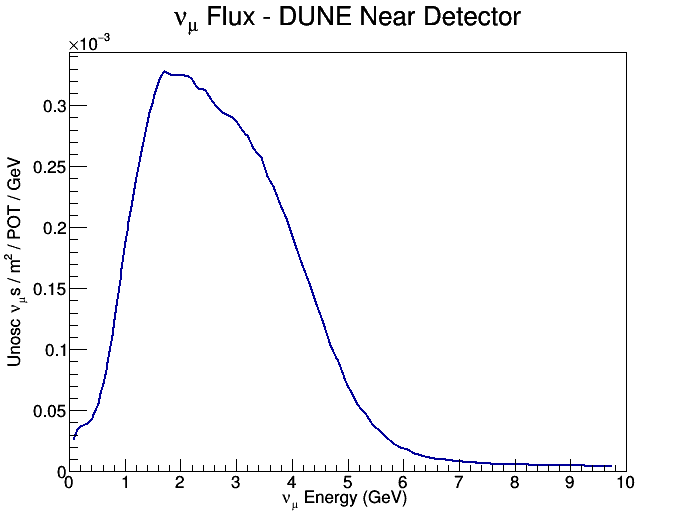
\includegraphics[width=\linewidth]{Dune_Flux/numu_ND_flux.png}
\endminipage
\minipage{.5\textwidth}
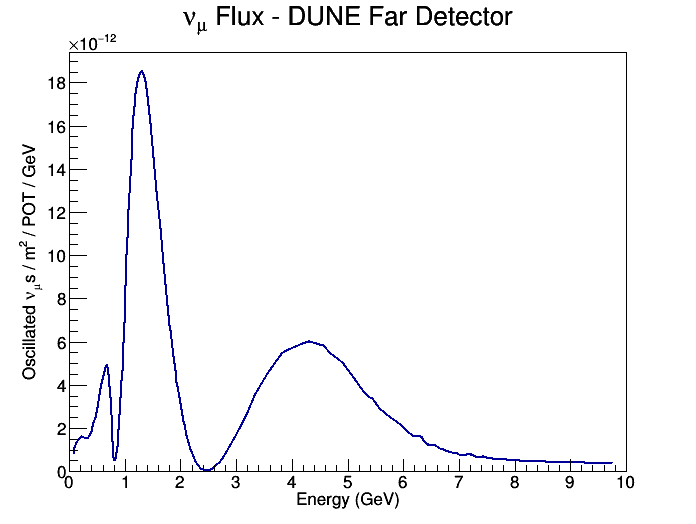
\includegraphics[width=\linewidth]{Dune_Flux/numu_FD_flux.png}
\endminipage
\caption{$\nu_\mu$ flux at DUNE ND (Left) and FD (Right)}
\label{fig:dune_flux}
\end{figure}

\begin{table}
\centering
 \begin{tabular}{| l  c  c |} 
 \hline 
 Parameter & Central Value & Relative Uncertainty\\ [0.5ex] 
 \hline
 $\theta_{12}$ & 0.5843 & 2.3\% \\ 
% \hline
 $\theta_{23}$ (NH) & 0.738 & 5.9\% \\
% \hline
 $\theta_{23}$ (IH) & 0.864 & 4.9\% \\
%  \hline
 $\theta_{13}$ & 0.148 & 2.5\% \\ 
% \hline
 $\Delta m^2_{21}$ & $7.5\times10^{-5} \textrm{eV}^2$ & 2.4\% \\
%  \hline
 $\Delta m^2_{31}$ (NH) & $2.457\times10^{-3} \textrm{eV}^2$ & 2.0\% \\
% \hline
 $\Delta m^2_{31}$ (IH) & $-2.449\times10^{-3} \textrm{eV}^2$ & 1.9\% \\[1ex]
% \hline
% 4 & 545 & 18744 \\
% \hline
% 5 & 88 & 788 \\ [1ex] 
 \hline
\end{tabular}
\caption{Oscillation parameters used for FD fluxes.}
\label{tab:osc}
\end{table}

\begin{table}
\centering
 \begin{tabular}{| l  c  |} 
 \hline 
 Event Type & Definiton\\ [0.5ex] 
 \hline
 True-CCQE & MC-level CCQE mode \\ 
% \hline
 True-2p2h & MC-level 2p2h mode \\
% \hline
 CC0$\pi$ & 0 $\pi^{\pm}$, 1 lepton, any number of protons and $\pi^0$ in final state. \\
%  \hline
 CC1$\pi$ & 1 $\pi^{\pm}$, 1 lepton, any number of protons and $\pi^0$ in final state. \\
% \hline
 CCOther & 1 lepton, any number of $\pi^{\pm}$, protons, and $\pi^0$ in final state. \\ [1ex]
 \hline
\end{tabular}
\caption{Definitions of various event types distinguished within our studies. Note that CCQE and 2p2h are based on MC-level reaction mode, but must also have 1 lepton in the final state if efficiencies are applied.}
\label{tab:events}
\end{table}


\FloatBarrier
	%All studies shown look at the effect of differences between the near and the far detector fluxes. However, we also include the different estimated efficiencies of each of the three near detector configurations.
\subsection{Near to Far Flux Comparisons}
\label{subsec:ntf}
The various studies regarding Near to Far extrapolations are explored using the following procedure. Ratios of either NEUT or NuWro to GENIE - referred to as 'single ratios' - separately at the ND and FD are taken. NEUT and NuWro are both normalized to GENIE to highlight shape differences rather than overall normalization effects. These offer insight into model variations and how the dependence of ND configuration couple to these variations.
The effect of a Near to Far extrapolation is approximated by taking a 'double ratio' between the near and far single ratios. To be explicit, these are defined in Equations ~\ref{eq:single_ratio} and ~\ref{eq:double_ratio}, where 'Other MC' refers to either NEUT or NuWro and 'Near' can be replaced by 'Far' in the single ratio. We note this is a crude approximation to give intuition about the problem for just a single reaction process; a fit to the ND spectrum will have multiple reactions in a given topology which can complicate the determination of physics effects for a single reaction.

\begin{equation}
\label{eq:single_ratio}
\textrm{ND Single Ratio} = \frac{\textrm{(Other MC @ Near Detector)}}{\textrm{(GENIE @ Near Detector)}}
\end{equation}

\begin{equation}
\label{eq:double_ratio}
\textrm{Double Ratio} = \frac{\textrm{(ND Single Ratio)}}{\textrm{(FD Single Ratio)}}
\end{equation}

Note that the studies in Section~\ref{subsec:N_multiplicities_Energy} use a slightly different Near to Far ratio, where the rates for a single generator is compared between ND and FD as in Figure~\ref{fig:Neutron_multi_2p2h_ND_FD}.
\subsection{Detector Configurations and Efficiencies}
\label{subsec:eff}
These studies highlight the effect of applying efficiencies of the various detectors. We first consider a 'perfect' ND and FD without any efficiencies applied, and then look what changes as we consider the 3 different configurations of the ND and a simple LAr efficiency in the FD. 

Efficiency information is included with the following procedure. Each particle is randomly accepted or rejected by throwing a random number and checking against the efficiency according to the particle's momentum. No angular efficiencies have yet been taken into account for this work. At the time of this writing, only a full description of the FGT efficiency according to NDTF samples is available, but other configurations will be added to subsequent versions of this note. An example of the efficiency for protons in the FGT is given in Figure~\ref{fig:FGT_proton_effs}; FGT efficiencies for other particles are included in Appendix~\ref{app:eff_app}. We also lack knowledge of the efficiencies for $\pi^0$ in the FGT, so we accept all of these in this configuration. Because we do not have the efficiencies for the LAr and GAr, simple thresholds for protons are applied for the GAr - 100 MeV/c - and LAr ND and FD - 200 MeV/c. We also make no assumptions for the efficiencies of $\mu$, $\pi^{+,-}$, and $\pi^{0}$ in the simple  descriptions, and so all of these types of particles are accepted in the LAr and GAr.

\begin{figure}[h]
\centering
\minipage{.5\textwidth}
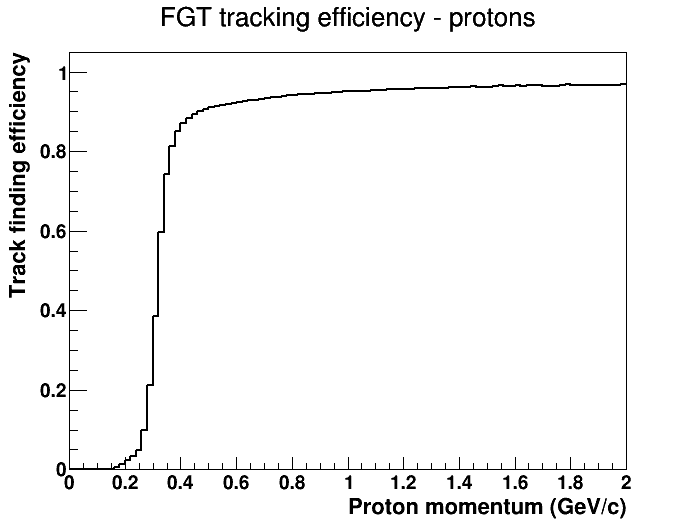
\includegraphics[width=\linewidth]{eff_plots/fgt_trkeff_proton.png}
\endminipage
\minipage{.5\textwidth}
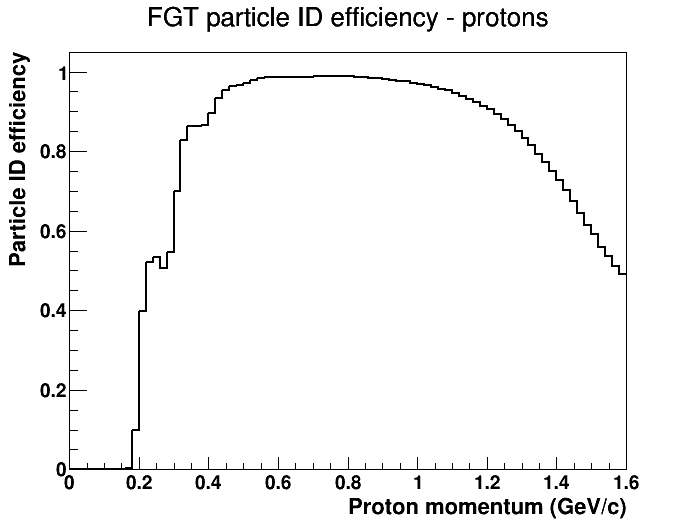
\includegraphics[width=\linewidth]{eff_plots/fgt_pideff_proton.png}
\endminipage
\caption{Left: Tracking efficiency for protons in FGT. Right: PID efficiency for protons in FGT. Total efficiency for a given proton momentum is given by the product of the two efficiencies.}
\label{fig:FGT_proton_effs}
\end{figure}


\section{Parameterization}
%The VALOR group\cite{VALOR} has led multiple T2K oscillation analyses and has contributed to most published T2K oscillation papers(I TOOK THIS ALMOST WORD FOR WORD FROM THE VALOR DOC BUT IDK WHAT TO WRITE FOR IT. IF CITING IT IS NOT GOOD ENOUGH I NEED TO CHANGE THIS). It also has contributed to to optimisation studies for DUNE, this being a source of motivation for this work. 
The VALOR software package has been used on multiple T2K oscillation analyses, and has recently been used to study the DUNE near detector configurations. %(((The group uses MC templates to map between reconstructed and true information for various reactions.))) 
The VALOR group has contributed to optimization studies for DUNE\cite{VALOR}, and has defined a $Q^2$ parameterization  - used to parameterize uncertainties according to model variations - for neutrinos and anti-neutrinos as: 
\begin{itemize}
\item CCQE $\nu_{\mu}$ with $Q^2$ bins \{0 - 0.20, 0.20 - 0.55, $>$0.55\} $\textrm{GeV}^2$
\item CCQE $\overline{\nu}_{\mu}$ with $Q^2$ bins \{0 - 0.20, 0.20 - 0.55, $>$0.55\} $\textrm{GeV}^2$
\item 2p2h $\nu_{\mu}$ with 1 $Q^2$ bin 
\item 2p2h $\overline{\nu}_{\mu}$ with 1 $Q^2$ bin
\end{itemize}

This portion of the work seeks to determine if variations in CCQE and 2p2h models are well represented by these parameterizations in $Q^2$. It also serves to highlight the behavior of the models as they couple to FSI and detector effect as we use a reconstructed $Q^2$ when efficiencies are applied. The variations are also studied in $q_0 \textrm{ vs. } q_3$ to check if a pure-$Q^2$ parameterization is sufficient.

\subsection{$Q^2$ Parameterization}
\label{subsec:q2}
%An obvious first step in the investigation of $Q^2$ parameterization sufficiency is to consider the relative change between the models and this change as it is extrapolated between the ND and FD Detector. 
The single and double ratio procedure described in Section~\ref{subsec:ntf} is conducted using events created by all three generators at the ND and FD and distributed according to $Q^2$. This is done separately with and without efficiencies, for both $\nu_{\mu}$ and $\overline{\nu}_{\mu}$, and for true-CCQE and true-2p2h. Applying efficiencies allows us to investigate how the interaction model can couple to detector effects. For distributions without efficiencies, the MC-level $Q^2$ quantity is used, giving us insight into the interaction model uncertainties. However, when including efficiencies, $Q^2$ becomes a reconstructed quantity, as it is calculated from the final state particles that are accepted after efficiencies are applied. This is highlighted in Equations~\ref{eq:Q2} - ~\ref{eq:ereco}. Though we call it 'reconstructed', it is calculated using the true energies and momentums without smearing applied, so it is not truly reconstructed in the usual sense of the word. Using this reconstructed quantity reveals how interaction/FSI variations, and detector acceptance effects couple together.

\begin{equation}
\label{eq:Q2}
Q^2 = |q_0^2 - q_3^2|,
\end{equation}
\begin{equation}
\label{eq:q0}
q_0^2 = (E_{reco} - E_{lep})^2,
\end{equation}
\begin{equation}
\label{eq:q3}
q_3^2 = (\vec{P}_{reco} - \vec{P}_{lep})^2
\end{equation}
\begin{equation}
E_{reco} =E_{lep} + \Sigma E_{\pi} + \Sigma (E_{prot} - M_{prot})
\label{eq:ereco}
\end{equation}

Conclusions are drawn from the double ratios according to the following prescription. We look for if the ratio is flat - i.e. if a horizontal line is within the statistical error bars - in a given bin of the parameterization. Flatness in that bin is a crude estimation for model-dependent shape uncertainties canceling out in a Near to Far extrapolation, and shows that a reweighting of that whole bin is sufficient to cover uncertainties. Again, we stress that this is a crude approximation to the Near to Far extrapolation.
 
%, true-2p2h, CC0$\pi^{\pm}$, CC1$\pi^{\pm}$, and CCOther as defined in Section~\ref{subsec:EDiff}

For $\nu_{\mu}$ CCQE events, both NEUT's and NuWro's models differ significantly from GENIE's model in $Q^2$ distributions, as seen in the single ratios in Figure~\ref{fig:Q2_ccqe_no_eff}. Despite this, the double ratios for both NEUT to GENIE and NuWro to GENIE remain relatively flat and close to 1, with small amounts of variation in the higher $Q^2$ region.

For double ratios with FGT efficiencies applied to the ND and simple LAr efficiencies applied to the FD, shape variations are greater above ~1.25 $\textrm{GeV}^2$ as seen in Figure~\ref{fig:Q2_ccqe_FGT_eff}. This suggests an additional bin in the region .55 to 1.25 $\textrm{GeV}^2$ should be included. These studies will be expanded in the future to increase statistics and determine the origin of the variation in this region, one possible source being the rejection of low-momentum muons after we apply efficiencies.

\begin{figure}[h]
\minipage{.32\textwidth}
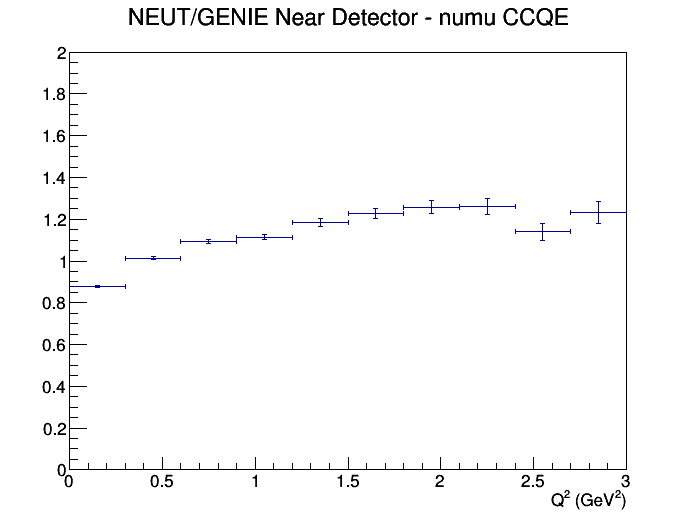
\includegraphics[width=\linewidth]{Q2/nominal/ratios/CCQE_NEUT_GENIE_numu_near_Q2.png}
\endminipage
\minipage{.32\textwidth}
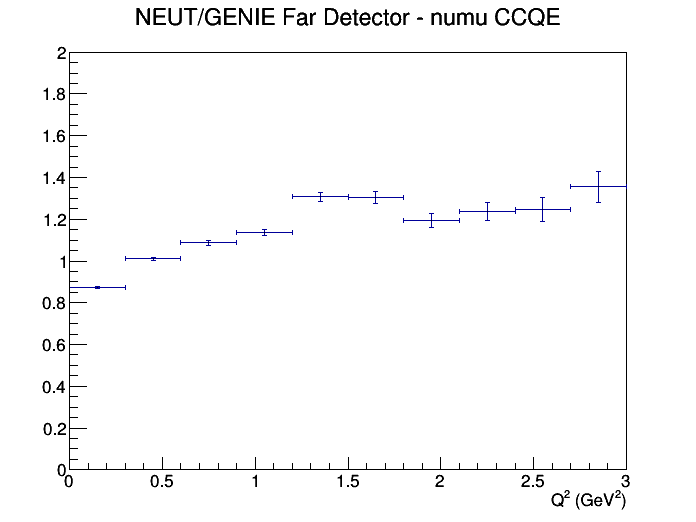
\includegraphics[width=\linewidth]{Q2/nominal/ratios/CCQE_NEUT_GENIE_numu_far_Q2.png}
\endminipage
\minipage{.32\textwidth}
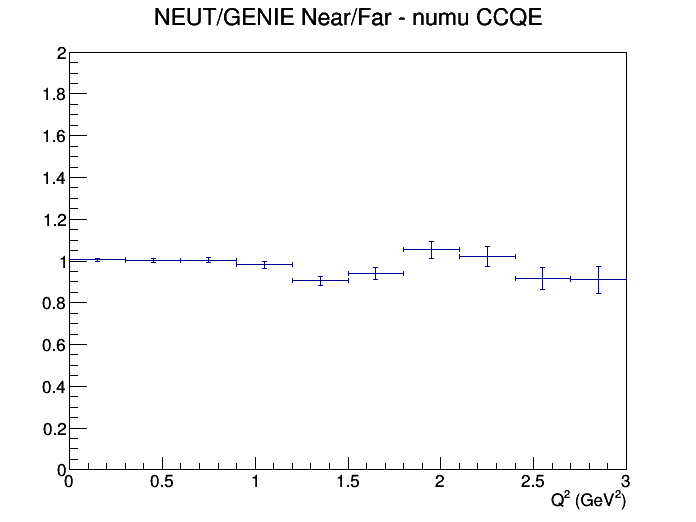
\includegraphics[width=\linewidth]{Q2/nominal/ratios/CCQE_NEUT_GENIE_numu_NF_Q2.png}
\endminipage
\newline
\minipage{.32\textwidth}
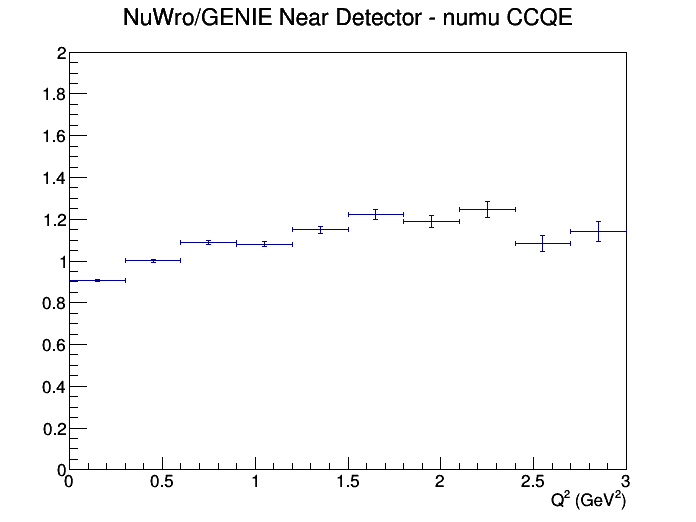
\includegraphics[width=\linewidth]{Q2/nominal/ratios/CCQE_NuWro_GENIE_numu_near_Q2.png}
\endminipage
\minipage{.32\textwidth}
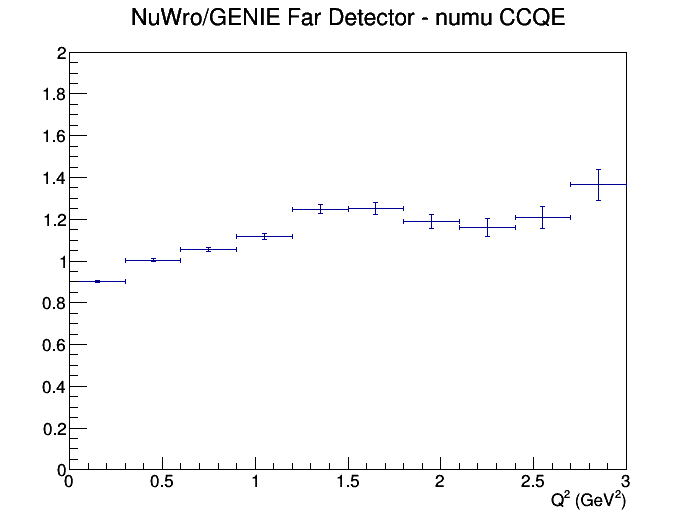
\includegraphics[width=\linewidth]{Q2/nominal/ratios/CCQE_NuWro_GENIE_numu_far_Q2.png}
\endminipage
\minipage{.32\textwidth}
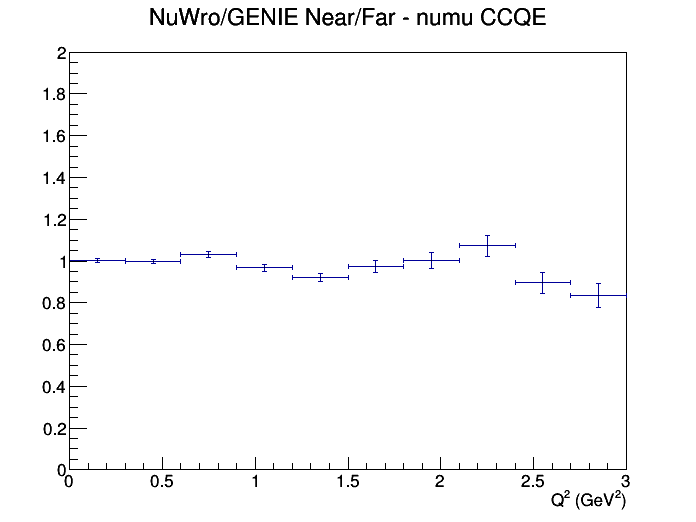
\includegraphics[width=\linewidth]{Q2/nominal/ratios/CCQE_NuWro_GENIE_numu_NF_Q2.png}
\endminipage
\caption{MC-level $Q^2$ distributed $\nu_{\mu}$ events using DUNE flux, no efficiencies applied to ND or FD. Top: Ratios of NEUT to GENIE. Bottom: Ratios of NuWro to GENIE. Left to Right: Single ratio at ND, single ratio at FD, double ratio Near/Far. Of note is the relative flatness throughout the double ratio compared to the single ratio at the ND. Note that the VALOR binning is separated by lower bin edges of (0, 0.20, and 0.55) $\textrm{GeV}^2$}
\label{fig:Q2_ccqe_no_eff}
\end{figure}
\begin{figure}[h]
\minipage{.32\textwidth}
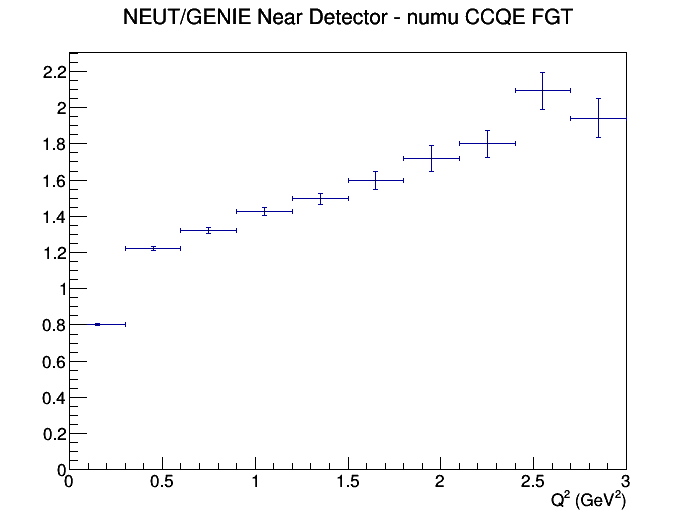
\includegraphics[width=\linewidth]{eff_Q2/FGT/ratios/CCQE_NEUT_GENIE_numu_near_Q2.png}
\endminipage
\minipage{.32\textwidth}
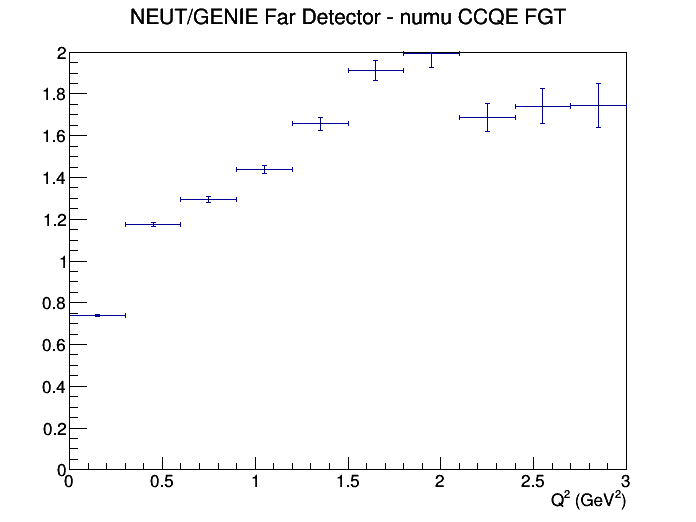
\includegraphics[width=\linewidth]{eff_Q2/FGT/ratios/CCQE_NEUT_GENIE_numu_far_Q2.png}
\endminipage
\minipage{.32\textwidth}
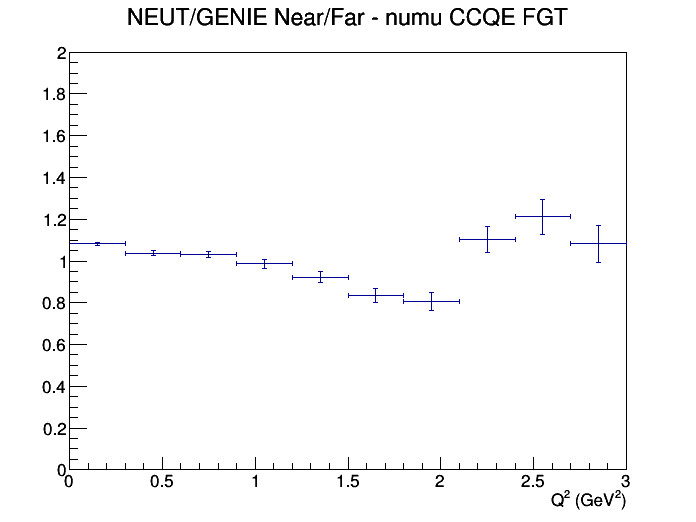
\includegraphics[width=\linewidth]{eff_Q2/FGT/ratios/CCQE_NEUT_GENIE_numu_NF_Q2.png}
\endminipage
\newline
\minipage{.32\textwidth}
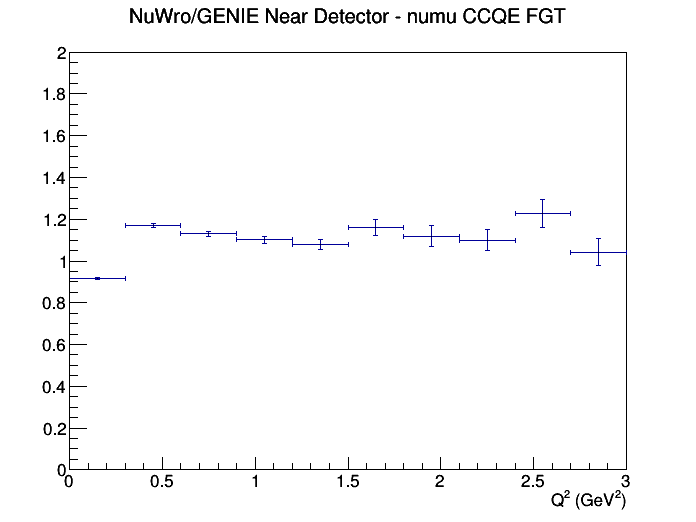
\includegraphics[width=\linewidth]{eff_Q2/FGT/ratios/CCQE_NuWro_GENIE_numu_near_Q2.png}
\endminipage
\minipage{.32\textwidth}
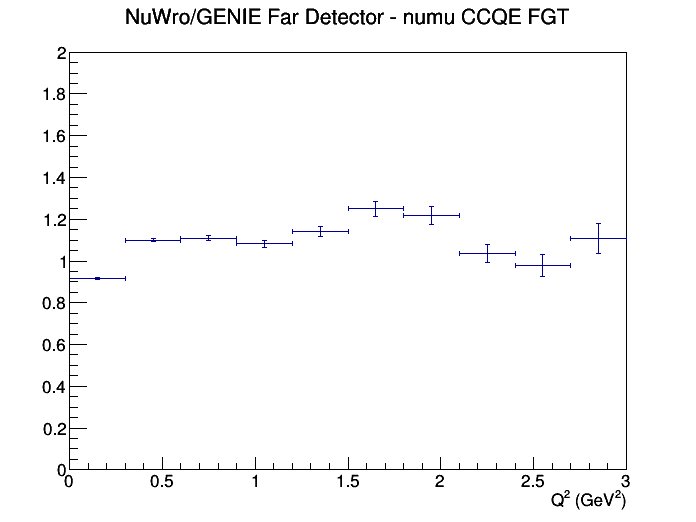
\includegraphics[width=\linewidth]{eff_Q2/FGT/ratios/CCQE_NuWro_GENIE_numu_far_Q2.png}
\endminipage
\minipage{.32\textwidth}
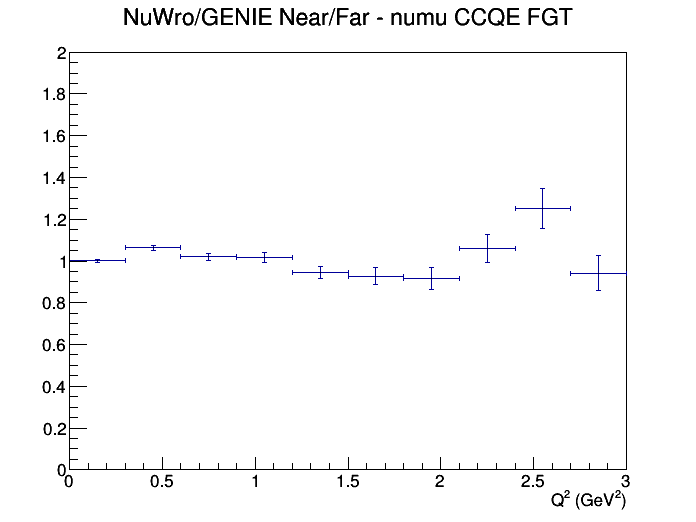
\includegraphics[width=\linewidth]{eff_Q2/FGT/ratios/CCQE_NuWro_GENIE_numu_NF_Q2.png}
\endminipage
\caption{Reconstructed $Q^2$ distributed $\nu_{\mu}$ events using DUNE flux, FGT efficiencies applied to ND and simple LAr efficiencies applied to FD. Top: Ratios of NEUT to GENIE. Bottom: Ratios of NuWro to GENIE. Left to Right: Single ratio at ND, single ratio at FD, double ratio Near/Far. More shape variations do arise above ~1.25 $\textrm{GeV}^2$ in the double ratios. This suggests another bin should encompass the region between .55 and 1.25 $\textrm{GeV}^2$. Note that the current VALOR binning is separated by lower bin edges of (0, 0.20, and 0.55) $\textrm{GeV}^2$}
\label{fig:Q2_ccqe_FGT_eff}
\end{figure}
\FloatBarrier


However, for $\overline{\nu}_{\mu}$ CCQE events, we observe distortions in the $Q^2$ distribution even in the double ratios. This is true without efficiencies for both NEUT to GENIE and NuWro to GENIE ratios. This is displayed in Figure~\ref{fig:Q2_ccqe_bar}. The variations again arise above 1.5 $\textrm{GeV}^2$ for the double ratios, supporting the addition of a bin between .55 and 1.25 $\textrm{GeV}^2$. This appears without efficiencies, and points to variations in the CCQE interaction model being responsible for this effect rather than FSI variations or detector effects.

We run into trouble extending the $\overline{\nu}_{\mu}$ CCQE study with efficiencies applied, as this leaves the high $Q^2$ region with very low statistics, preventing us from drawing any meaningful conclusions. These plots are included in Appendix~\ref{app:Q2_app} for completeness. The studies will be continued once we have higher statistics, and with more complete descriptions of the LAr and GAr as this information becomes available.

\begin{figure}[h]
\minipage{.32\textwidth}
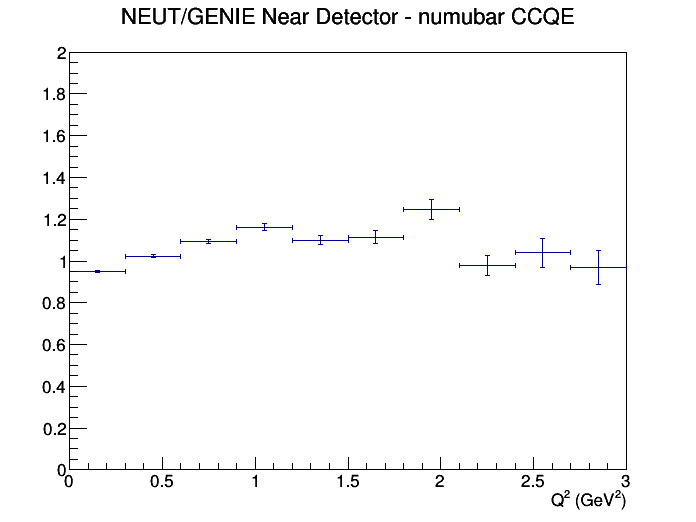
\includegraphics[width=\linewidth]{Q2/nominal/ratios/CCQE_NEUT_GENIE_numubar_near_Q2.png}
\endminipage
\minipage{.32\textwidth}
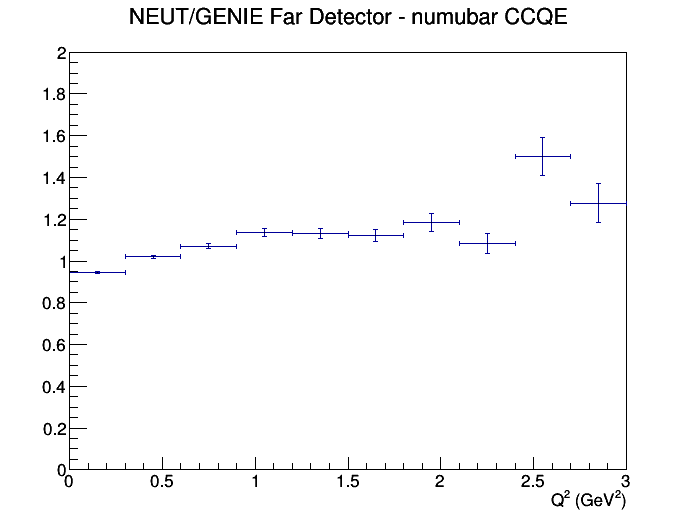
\includegraphics[width=\linewidth]{Q2/nominal/ratios/CCQE_NEUT_GENIE_numubar_far_Q2.png}
\endminipage
\minipage{.32\textwidth}
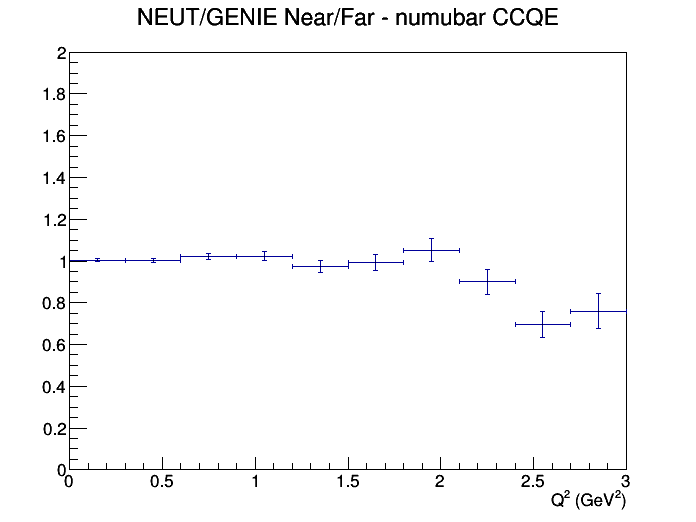
\includegraphics[width=\linewidth]{Q2/nominal/ratios/CCQE_NEUT_GENIE_numubar_NF_Q2.png}
\endminipage
\newline
\minipage{.32\textwidth}
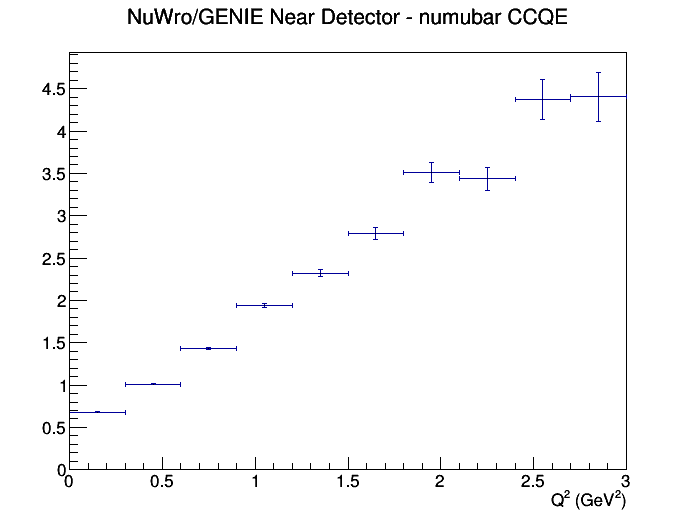
\includegraphics[width=\linewidth]{Q2/nominal/ratios/CCQE_NuWro_GENIE_numubar_near_Q2.png}
\endminipage
\minipage{.32\textwidth}
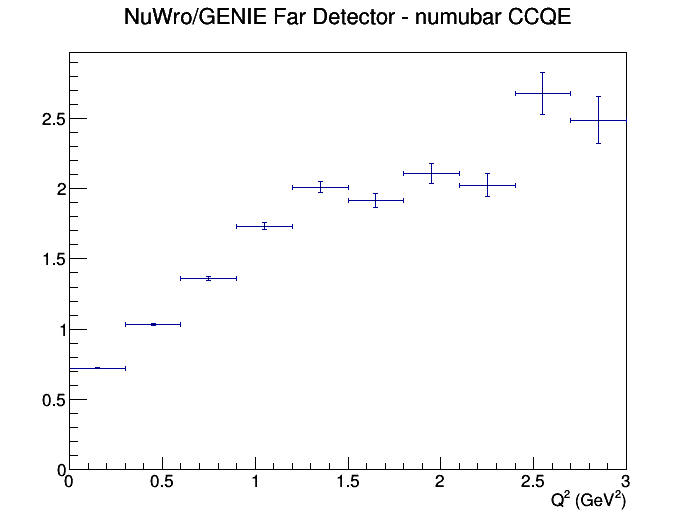
\includegraphics[width=\linewidth]{Q2/nominal/ratios/CCQE_NuWro_GENIE_numubar_far_Q2.png}
\endminipage
\minipage{.32\textwidth}
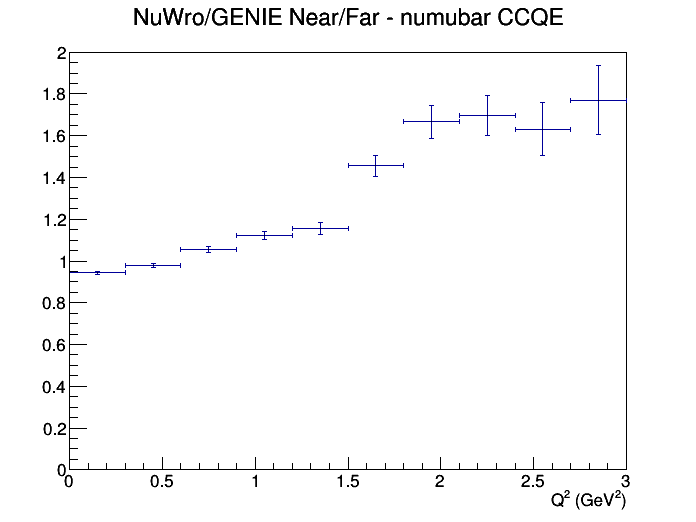
\includegraphics[width=\linewidth]{Q2/nominal/ratios/CCQE_NuWro_GENIE_numubar_NF_Q2.png}
\endminipage
\caption{MC-level $Q^2$ distributed $\overline{\nu}_{\mu}$ CCQE events using DUNE flux. Top: Ratios of NEUT to GENIE. Bottom: Ratios of NuWro to GENIE. Left to Right: Single ratio at ND, single ratio at FD, double ratio Near/Far. Large amounts of variations in the region above 1.5 $\textrm{GeV}^2$ in both double ratios. This differs from $\nu_{\mu}$ CCQE, where this arose in the ratios after efficiencies are added. Here, it exists without any efficiencies. This points to variations in the CCQE model, rather than FSI or detector effects, not being covered by the parameterization. An additional bin between .55 and 1.25 $\textrm{GeV}^2$ is suggested. Note that the VALOR binning is separated by lower bin edges of (0, 0.20, and 0.55) $\textrm{GeV}^2$.}
\label{fig:Q2_ccqe_bar}
\end{figure}
\FloatBarrier

For 2p2h $\nu_{\mu}$ and $\overline{\nu}_{\mu}$ events, the double ratios from both NEUT and NuWro remain centered close to or around 1 below about 1 $\textrm{GeV}^2$ without efficiencies applied, as seen in Figure~\ref{fig:Q2_2p2h_numu_no_eff} and ~\ref{fig:Q2_2p2h_numubar_no_eff}. Above 1 $\textrm{GeV}^2$, the statistics are again low. At this moment, the currently-proposed 1-bin normalization appears sufficient in the region below 1 $\textrm{GeV}^2$. The low statistics prevent us from making conclusions in the high $Q^2$ region as well as drawing conclusions from applying efficiencies. These will be revisited in later iterations of this work.
\begin{figure}[h]
\minipage{.32\textwidth}
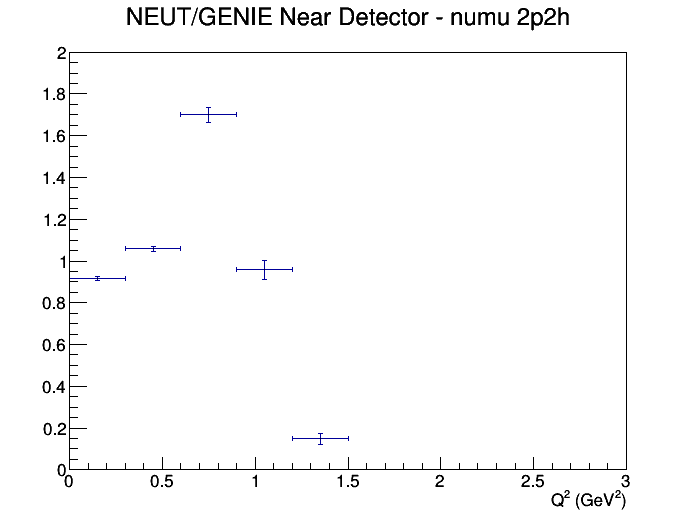
\includegraphics[width=\linewidth]{Q2/nominal/ratios/2p2h_NEUT_GENIE_numu_near_Q2.png}
\endminipage
\minipage{.32\textwidth}
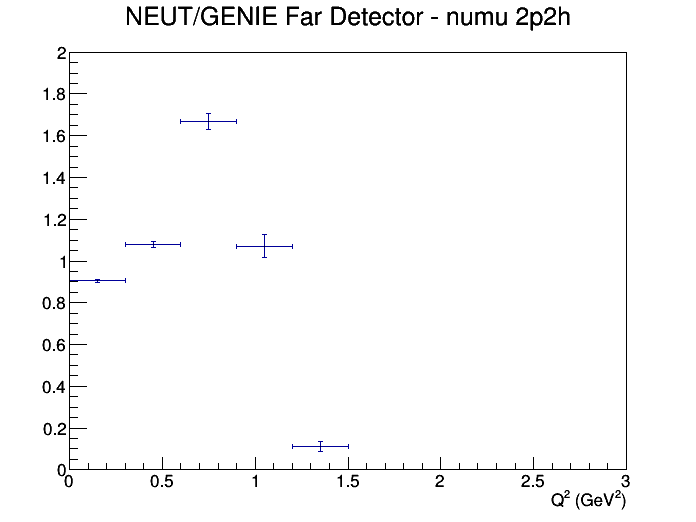
\includegraphics[width=\linewidth]{Q2/nominal/ratios/2p2h_NEUT_GENIE_numu_far_Q2.png}
\endminipage
\minipage{.32\textwidth}
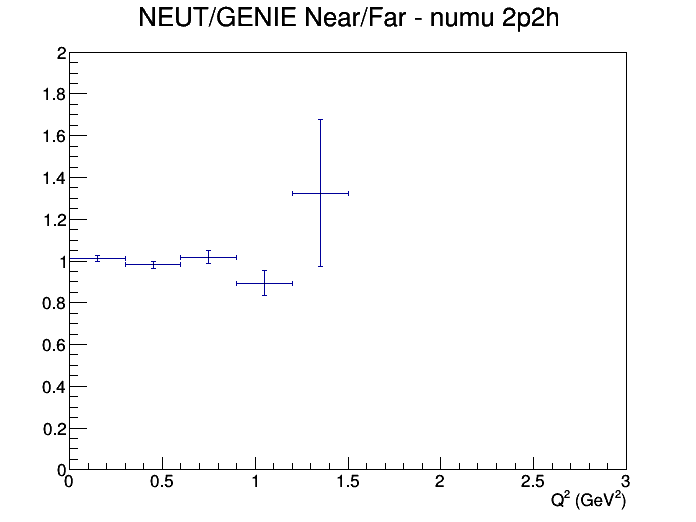
\includegraphics[width=\linewidth]{Q2/nominal/ratios/2p2h_NEUT_GENIE_numu_NF_Q2.png}
\endminipage
\newline
\minipage{.32\textwidth}
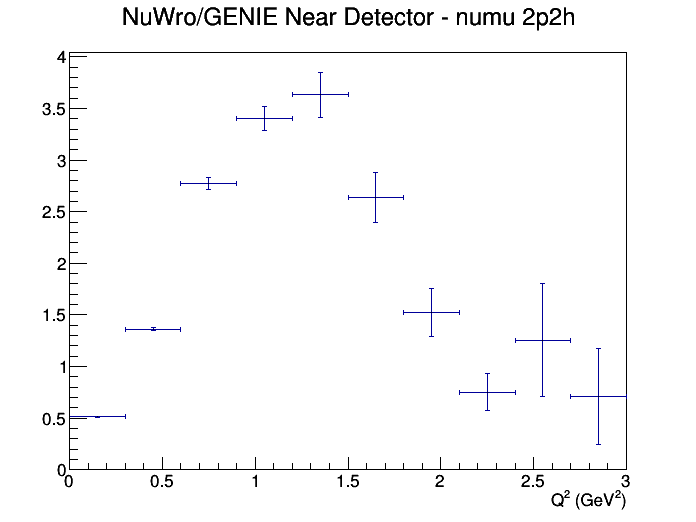
\includegraphics[width=\linewidth]{Q2/nominal/ratios/2p2h_NuWro_GENIE_numu_near_Q2.png}
\endminipage
\minipage{.32\textwidth}
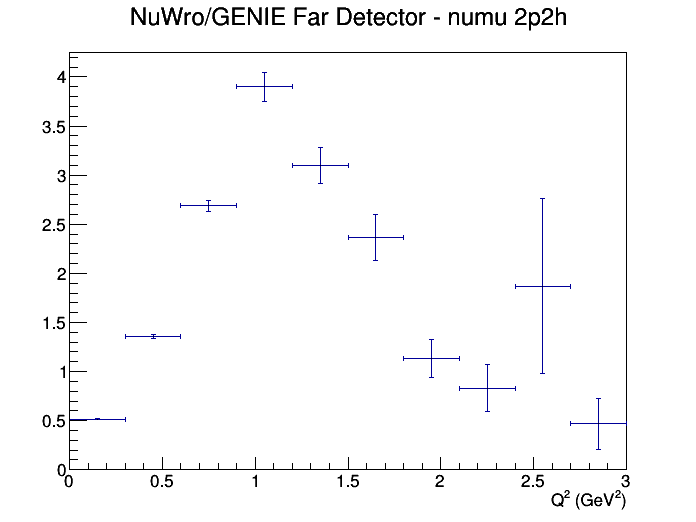
\includegraphics[width=\linewidth]{Q2/nominal/ratios/2p2h_NuWro_GENIE_numu_far_Q2.png}
\endminipage
\minipage{.32\textwidth}
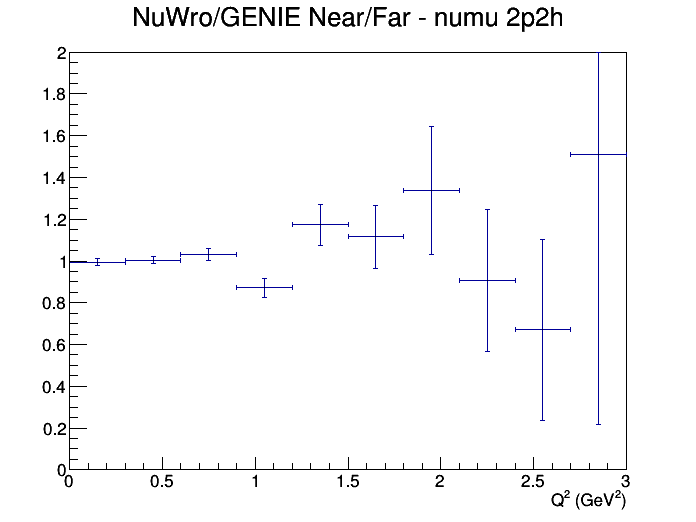
\includegraphics[width=\linewidth]{Q2/nominal/ratios/2p2h_NuWro_GENIE_numu_NF_Q2.png}
\endminipage
\caption{$Q^2$ distributed $\overline{\nu}_{\mu}$ 2p2h events using DUNE flux. Top: Ratios of NEUT to GENIE. Bottom: Ratios of NuWro to GENIE. Left to Right: Single ratio at ND, single ratio at FD, double ratio Near/Far. Large amounts of variations are present resulting from low statistics in the higher end of all distributions, but the lower end holds close to 1. Note that the VALOR binning is separated by lower bin edges of (0, 0.20, and 0.55) $\textrm{GeV}^2$.}
\label{fig:Q2_2p2h_numu_no_eff}
\end{figure}

\begin{figure}[h]
\minipage{.32\textwidth}
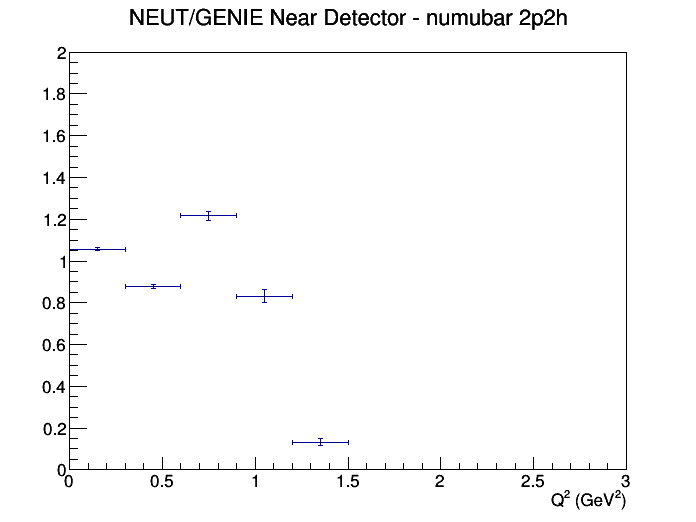
\includegraphics[width=\linewidth]{Q2/nominal/ratios/2p2h_NEUT_GENIE_numubar_near_Q2.png}
\endminipage
\minipage{.32\textwidth}
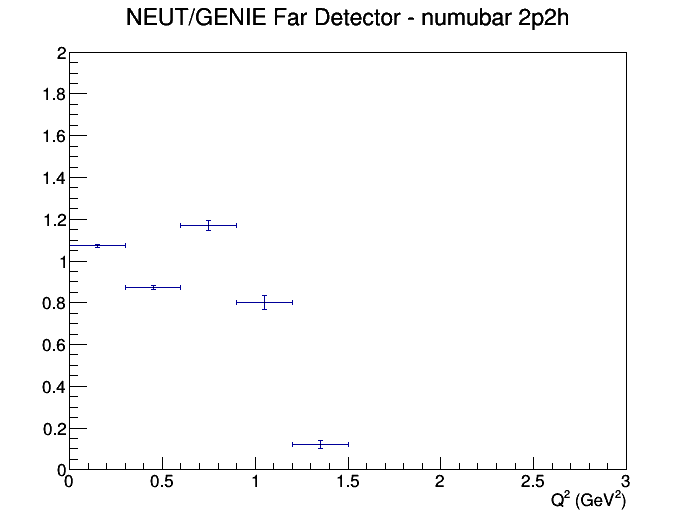
\includegraphics[width=\linewidth]{Q2/nominal/ratios/2p2h_NEUT_GENIE_numubar_far_Q2.png}
\endminipage
\minipage{.32\textwidth}
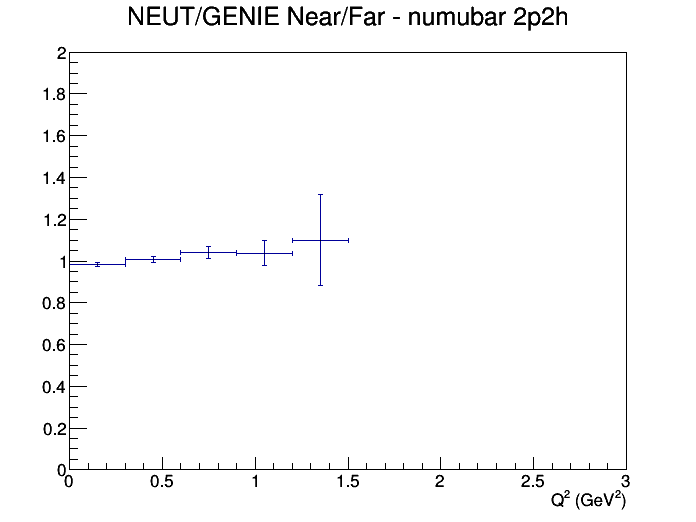
\includegraphics[width=\linewidth]{Q2/nominal/ratios/2p2h_NEUT_GENIE_numubar_NF_Q2.png}
\endminipage
\newline
\minipage{.32\textwidth}
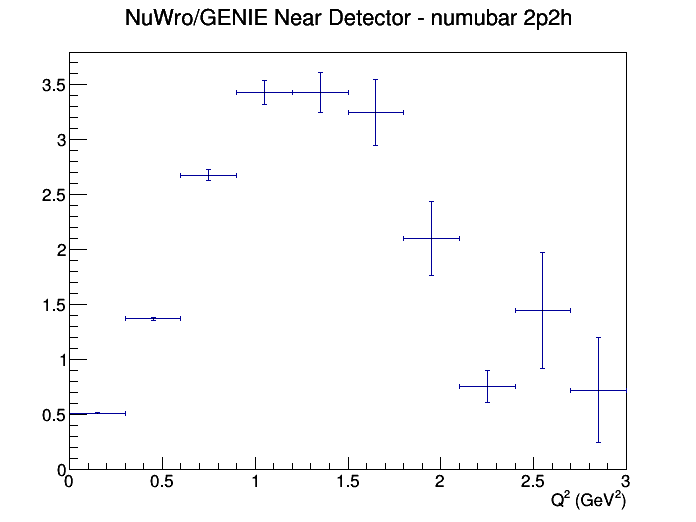
\includegraphics[width=\linewidth]{Q2/nominal/ratios/2p2h_NuWro_GENIE_numubar_near_Q2.png}
\endminipage
\minipage{.32\textwidth}
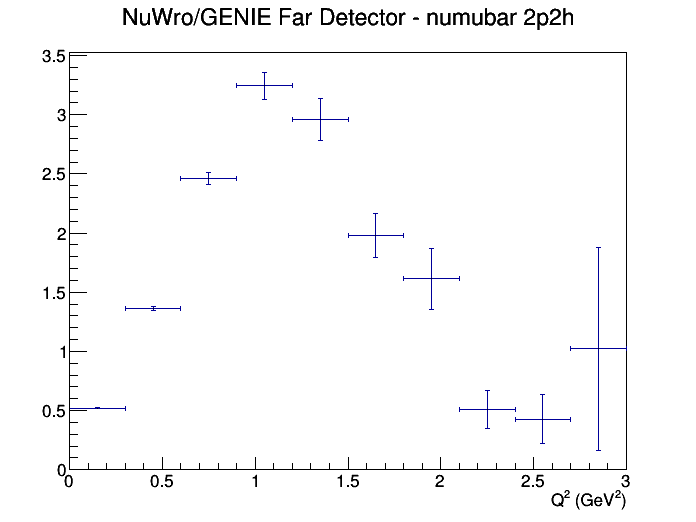
\includegraphics[width=\linewidth]{Q2/nominal/ratios/2p2h_NuWro_GENIE_numubar_far_Q2.png}
\endminipage
\minipage{.32\textwidth}
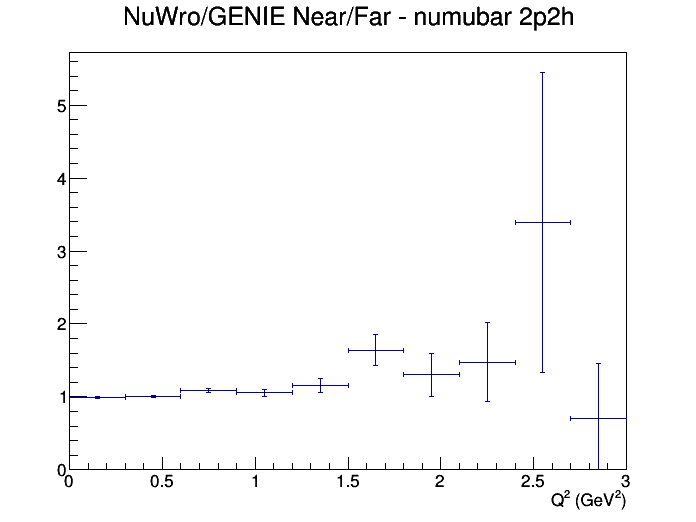
\includegraphics[width=\linewidth]{Q2/nominal/ratios/2p2h_NuWro_GENIE_numubar_NF_Q2.png}
\endminipage
\caption{$Q^2$ distributed $\overline{\nu}_{\mu}$ 2p2h events using DUNE flux. Top: No efficiencies, Bottom: FGT efficiencies applied to ND, LAr efficiencies applied to FD. Left to right: NEUT to GENIE double ratio, NuWro to GENIE double ratio. Large amounts of deviations from 1 throughout distributions with efficiencies applied. Note that the VALOR binning is separated by lower bin edges of (0, 0.20, and 0.55) $\textrm{GeV}^2$.}
\label{fig:Q2_2p2h_numubar_no_eff}
\end{figure}
\FloatBarrier

We currently find an additional bin in the region (.55, ~1.25) will account for uncertainties in both $\nu_{\mu}$ and $\overline{\nu}_{\mu}$ CCQE. For $\nu_{\mu}$ and $\overline{\nu}_{\mu}$ 2p2h, the overall normalization currently appears sufficient from these studies. Investigations into the origin of the variation in the high $Q^2$ region of CCQE will be conducted as this work is furthered. Additional statistics and more complete efficiency descriptions for the LAr and GAr are required, and will be conducted at a later date.

\subsection{$q_0 \textrm{ vs. } q_3$ Variations}
\label{subsec:q0q3}
In addition to studying the $Q^2$ ratios, the ratios in $q_0 \textrm{ - } q_3$ were also investigated to explore the possibility that variations arise when changing the parameterization from $Q^2$ to $q_0 \textrm{ - } q_3$. The $Q^2$ parameterization assumes the variations are purely functions of $Q^2$. Under this assumption, the double ratios should be flat in $q_0 \textrm{ - } q_3$ regions corresponding to the $Q^2$-binned parameterization. If this is not the case, a pure-$Q^2$ parameterization cannot sufficiently account for CCQE and 2p2h variations.

These studies were done in the exact same way as those in the previous section, only with the events and ratios distributed in $q_0 \textrm{ - } q_3$ bins. Note: to be symmetric around 1, the scale extends from 0 to 2, but the variations in those bins can actually be greater than 2. Again, the quantities are MC-level truth information in the distributions without efficiencies, but are reconstructed in those with efficiencies applied, as described in Equations~\ref{eq:Q2} - ~\ref{eq:ereco}.

For $\nu_{\mu}$ CCQE, the double ratios without efficiencies appear flat for both NEUT to GENIE and NuWro to GENIE double ratios, as seen in Figure~\ref{fig:q0q3_numu_CCQE_no_eff}. There is distortion in the upper right region, consistent with the high $Q^2$ regions in Figure~\ref{fig:Q2_ccqe_no_eff}.  This binning proves to be a problem for creating reliable conclusions once efficiencies are applied, as statistics for each individual bin become quite low. These are included in Appendix~\ref{app:q0q3_app}. Higher statistics will be achieved for future work.
%\newline
\begin{figure}[h]
\centering
\minipage{.5\textwidth}
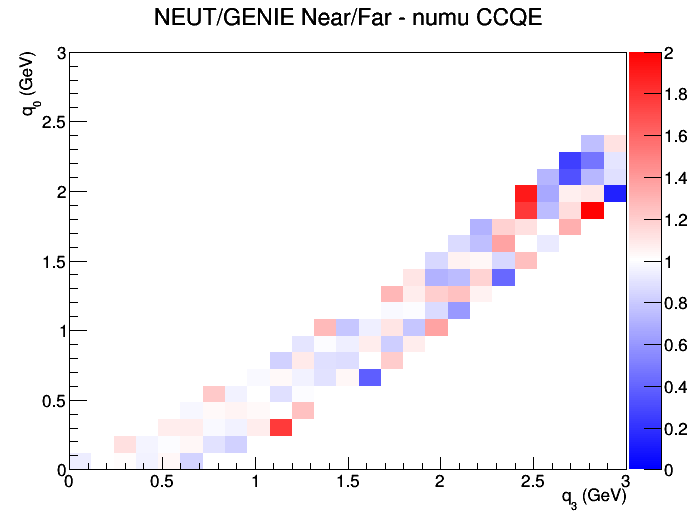
\includegraphics[width=\linewidth]{q0_q3/nominal/ratios/CCQE_NEUT_GENIE_numu_NF_q3_q0.png}
\endminipage
\minipage{.5\textwidth}
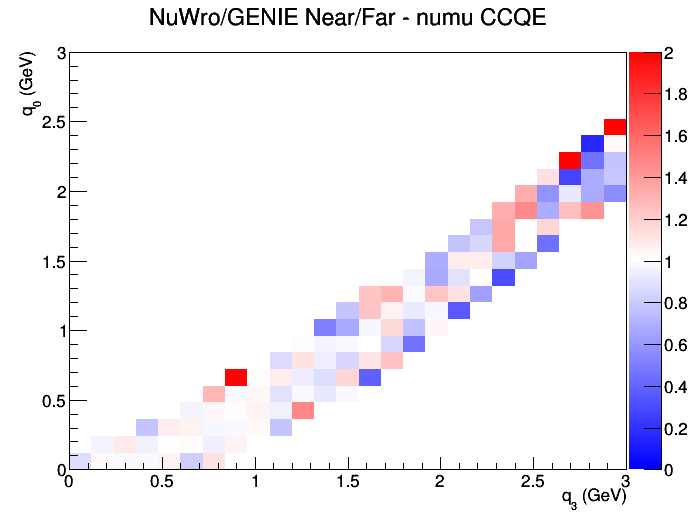
\includegraphics[width=\linewidth]{q0_q3/nominal/ratios/CCQE_NuWro_GENIE_numu_NF_q3_q0.png}
\endminipage
\caption{MC-level $q_0 \textrm{ - } q_3$ distributed $\nu_{\mu}$ CCQE events using DUNE flux without efficiencies applied. Left: Double ratio of NEUT to GENIE, Right: Double ratio of NuWro to GENIE. Relatively flat distributions, but with bin-to-bin variations arising from low statistics. Consistent with corresponding $Q^2$ ratios} 
\label{fig:q0q3_numu_CCQE_no_eff}
\end{figure}
\FloatBarrier

For $\overline{\nu}_{\mu}$ CCQE, the large variations in the high $Q^2$ region are present in the corresponding $q_0 \textrm{ - } q_3$ region. As shown in Figure~\ref{fig:q0q3_numubar_CCQE_no_eff}, the upper right region of both double ratios are consistent with the corresponding double ratios in Figure~\ref{fig:Q2_ccqe_bar}. Here again, the NuWro to GENIE double ratio is consistently higher in this region, while the NEUT to GENIE double ratio is slightly lower.

\begin{figure}[h]
\centering
\minipage{.5\textwidth}
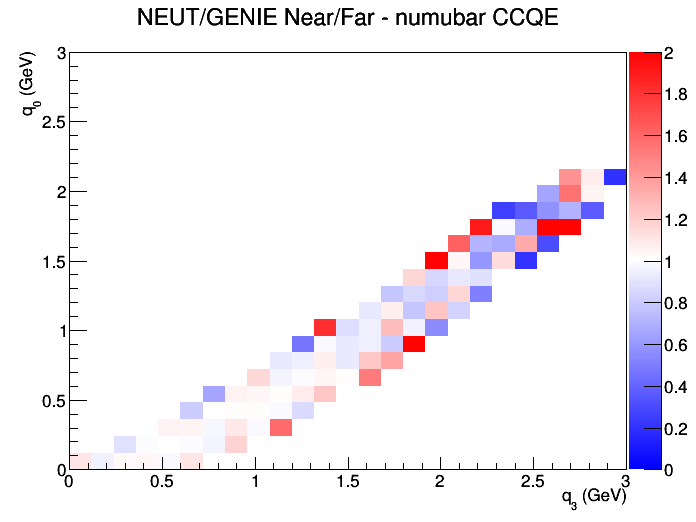
\includegraphics[width=\linewidth]{q0_q3/nominal/ratios/CCQE_NEUT_GENIE_numubar_NF_q3_q0.png}
\endminipage
\minipage{.5\textwidth}
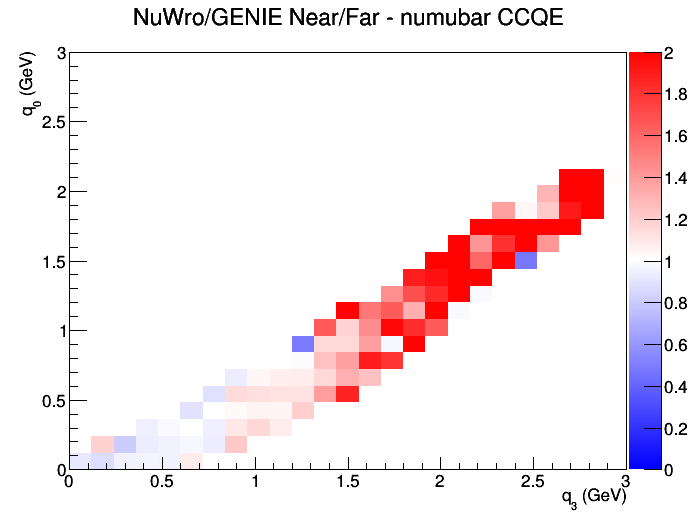
\includegraphics[width=\linewidth]{q0_q3/nominal/ratios/CCQE_NuWro_GENIE_numubar_NF_q3_q0.png}
\endminipage
\caption{$q_0 \textrm{ - } q_3$ distributed $\overline{\nu}_{\mu}$ CCQE events using DUNE flux without efficiencies applied. Left: Double ratio of NEUT to GENIE, Right: Double ratio of NuWro to GENIE. Variations in upper right region are consistent with corresponding $Q^2$ ratios.}
\label{fig:q0q3_numubar_CCQE_no_eff}
\end{figure}
\FloatBarrier

Each of the three generators have very different behavior for 2p2h $\nu_\mu$ and $\overline{\nu}_{\mu}$ events with no efficiencies applied, as can be seen in Figure~\ref{fig:q0q3_2p2h_events}. This contains the raw event rate for 2p2h, and is shown to highlight the drastic shape difference. This causes very restricted phase space in the double ratios in $q_0 \textrm{ - } q_3$, and so double ratios are not shown here - however they are included in Appendix ~\ref{app:q0q3_app}. The shape differences suggest that an overall binning in $Q^2$ cannot cover uncertainties, and reweighting events according to $q_0 \textrm{ - } q_3$ shape should be used instead.
\begin{figure}[h]
\centering
\minipage{.32\textwidth}
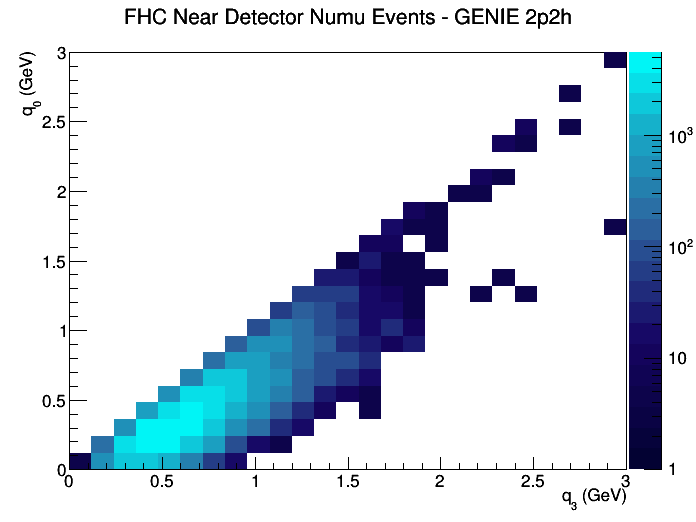
\includegraphics[width=\linewidth]{q0_q3/nominal/2p2h_FHC_ND_numu_q3_q0_GENIE.png}
\endminipage
\minipage{.32\textwidth}
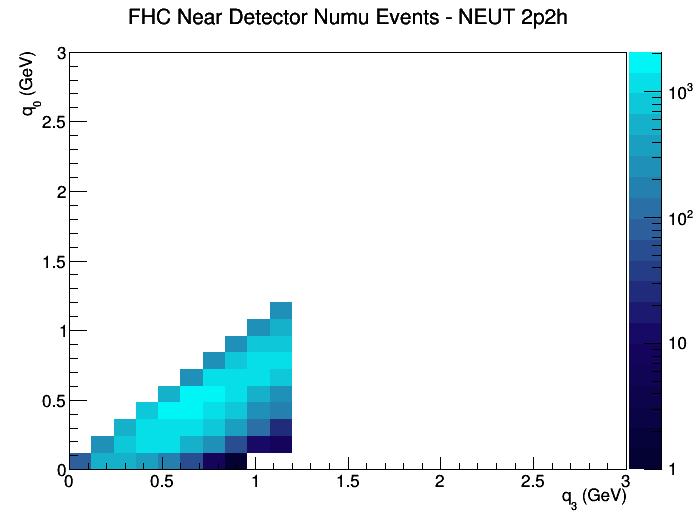
\includegraphics[width=\linewidth]{q0_q3/nominal/2p2h_FHC_ND_numu_q3_q0_NEUT.png}
\endminipage
\minipage{.32\textwidth}
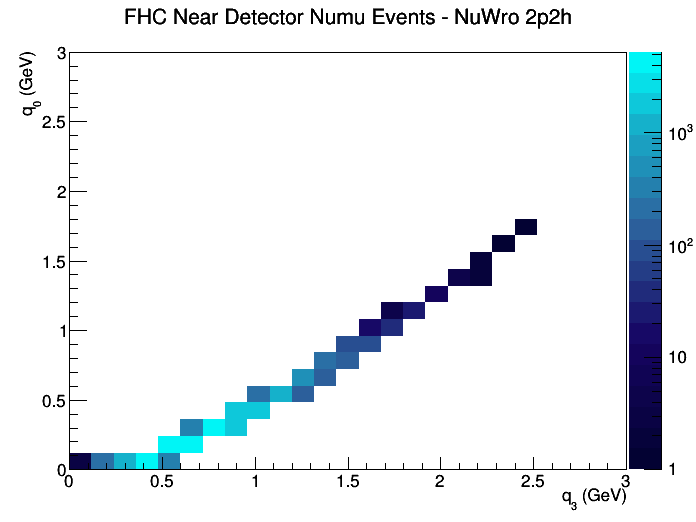
\includegraphics[width=\linewidth]{q0_q3/nominal/2p2h_FHC_ND_numu_q3_q0_NuWro.png}
\endminipage
\newline
\minipage{.32\textwidth}
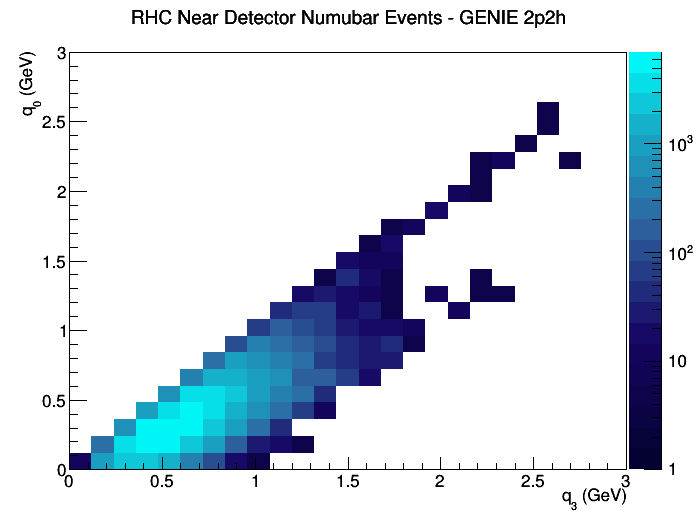
\includegraphics[width=\linewidth]{q0_q3/nominal/2p2h_RHC_ND_numubar_q3_q0_GENIE.png}
\endminipage
\minipage{.32\textwidth}
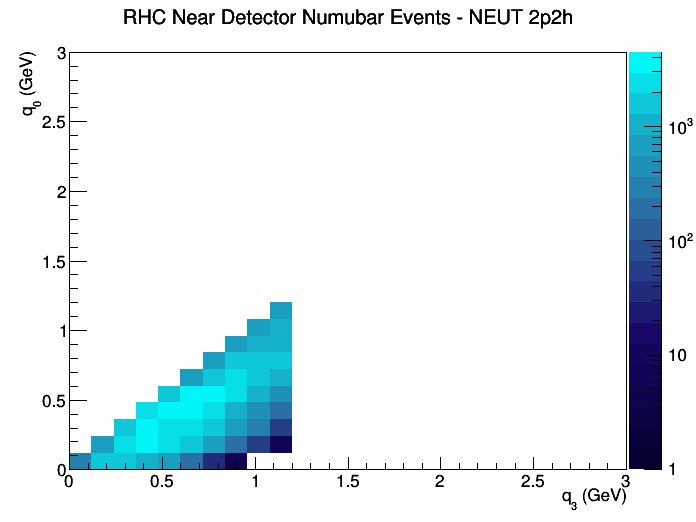
\includegraphics[width=\linewidth]{q0_q3/nominal/2p2h_RHC_ND_numubar_q3_q0_NEUT.png}
\endminipage
\minipage{.32\textwidth}
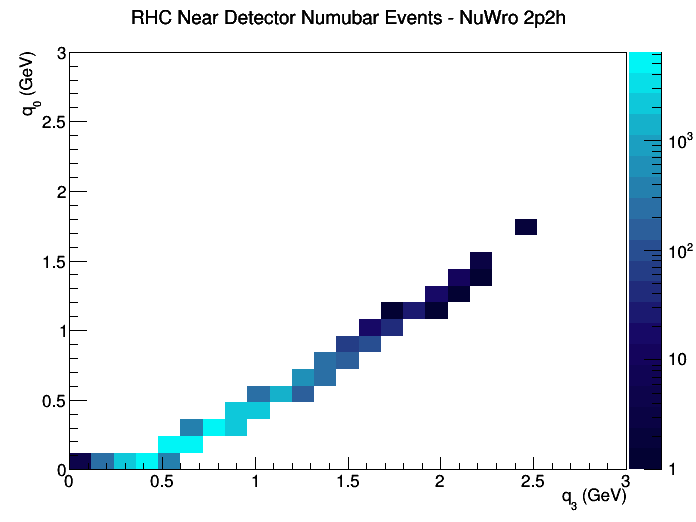
\includegraphics[width=\linewidth]{q0_q3/nominal/2p2h_RHC_ND_numubar_q3_q0_NuWro.png}
\endminipage
\caption{MC-level $q_0 \textrm{ - } q_3$ distributed 2p2h events using DUNE flux with no efficiencies applied. Top: $\nu_{\mu}$ events, Bottom: $\overline{\nu}_{\mu}$ events. Right to Left: GENIE events distribution, NEUT events distribution, NuWro events distribution. The phase spaces are very different without efficiencies, and restrict the coverage of the double ratios in $q_0 \textrm{ - } q_3$. This suggests the use of 1 $Q^2$ is insufficient bin to cover uncertainties.}
\label{fig:q0q3_2p2h_events}
\end{figure}
\FloatBarrier

\subsection{Parameterization - Conclusions}
It appears as though the pure-$Q^2$ parameterization and the binning developed by VALOR would cover model variations for $\nu_{\mu}$ and $\overline{\nu}_{\mu}$ CCQE events, but slight modifications are suggested. The Near to Far extrapolation plots - the double ratios - appear relatively flat in the regions of the individual bins in the low $Q^2$ region. This changes above ~1.25 $\textrm{GeV}^2$, so placing another bin between 0.55 and ~1.25 $\textrm{GeV}^2$ should suffice. The $q_0 \textrm{ - } q_3$ double ratios are consistent with this conclusion. Future work will be focused on improving statistics and implementing full LAr and GAr efficiencies as that information becomes available, as well as investigating the origin of the high-$Q^2$ variations which possibly arise from proton or - more-likely - muon acceptance effects. 

The low-$Q^2$ $\nu_{\mu}$ and $\overline{\nu}_{\mu}$ 2p2h events appear to be covered by the current 1-bin parameterization when only looking at the $Q^2$ distribution. However, the shape differences in $q_0 \textrm{ - } q_3$ show that a pure-$Q^2$ parameterization should not be used. Future work will continue with improving statistics, as well as implementing all efficiencies.

%There is a degree of statistical limitation of the studies at this point, evident in the presence of bin-to-bin variations. To explore this point further, these studies can quickly and easily be extended to larger data sets to deal with statistics limitations. Additionally, the statistical uncertainties in the single and double ratios will also be investigated. With these, we can move on to quantify the degree to which the near-to-far extrapolation covers variations in the $\nu_{\mu}$ case - or does not cover variations in the $\overline{\nu}_{\mu}$ case. 

%For the rest of the reaction modes, the trend - that $\nu_{\mu}$ ratios appear to be relatively flat for both NEUT and NuWro, while $\overline{\nu}_{\mu}$ NuWro to GENIE double ratio is noticeably greater than 1 - continues. This can be seen in Appendix~\ref{app:q0q3_app}. Of note, however, is the shape of $\nu_\mu$ and $\overline{\nu}_{\mu}$ CCOther events before and after efficiencies are applied in each generator. As shown in Figure~\ref{fig:q0q3_numu_CCOther_events}, the left region of $q_0 \textrm{ - } q_3$ space is empty before efficiencies, but is filled in after efficiencies are applied. This corresponds to a low $Q^2$ region, which is shown to be filled in after efficiencies in the $Q^2$ distribution in Figure~\ref{fig:Q2_numu_CCOther_events}.
%\begin{figure}[h]
%\centering
%\minipage{.3\textwidth}
%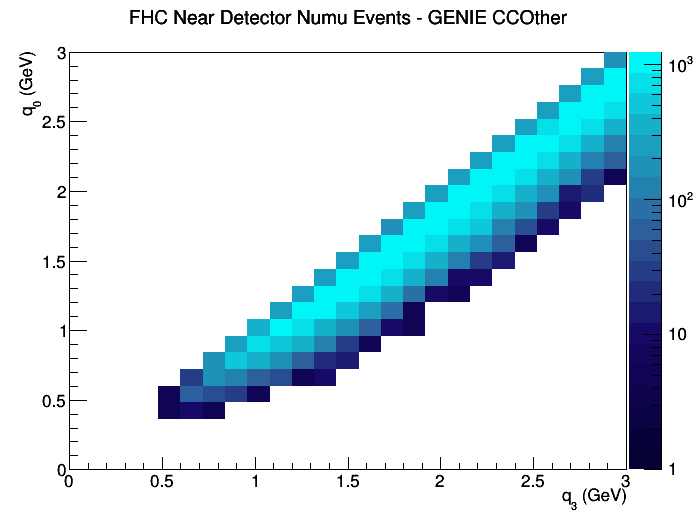
\includegraphics[width=\linewidth]{q0_q3/nominal/CCOther_FHC_ND_numu_q3_q0_GENIE.png}
%\endminipage
%\minipage{.3\textwidth}
%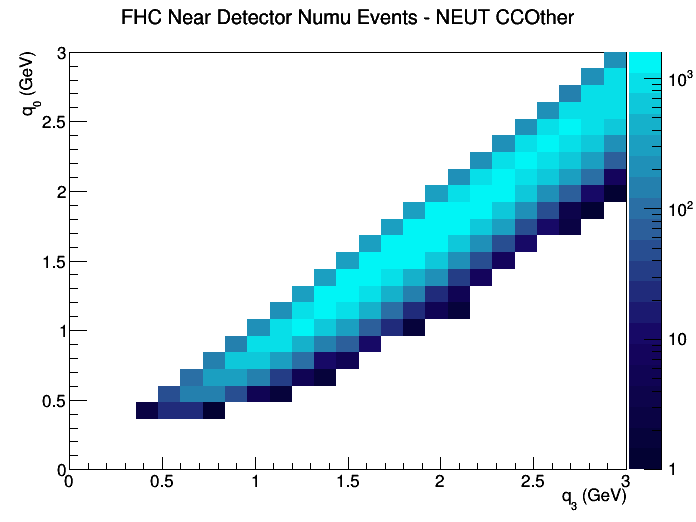
\includegraphics[width=\linewidth]{q0_q3/nominal/CCOther_FHC_ND_numu_q3_q0_NEUT.png}
%\endminipage
%\minipage{.3\textwidth}
%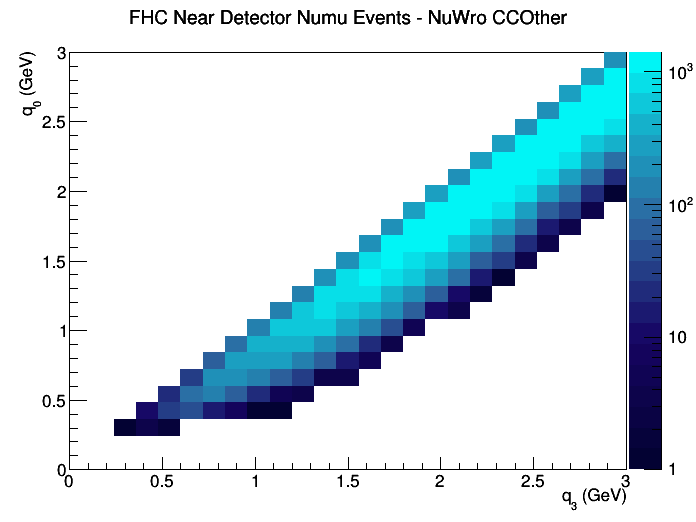
\includegraphics[width=\linewidth]{q0_q3/nominal/CCOther_FHC_ND_numu_q3_q0_NuWro.png}
%\endminipage
%\newline
%\minipage{.3\textwidth}
%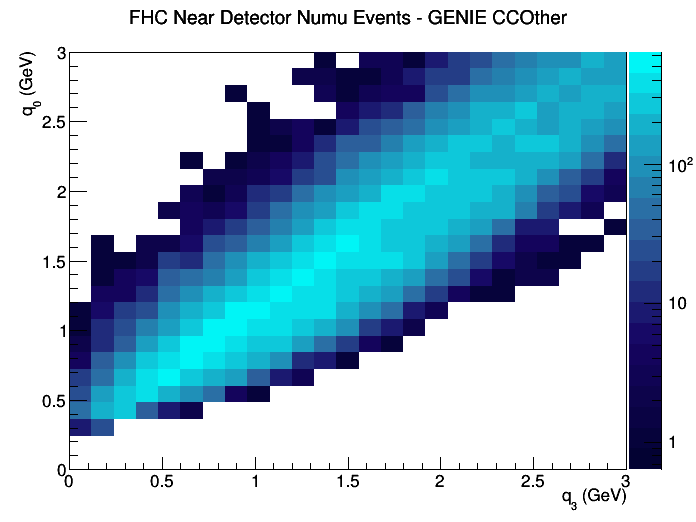
\includegraphics[width=\linewidth]{eff_q0_q3/FGT/CCOther_FHC_ND_numu_q3_q0_GENIE.png}
%\endminipage
%\minipage{.3\textwidth}
%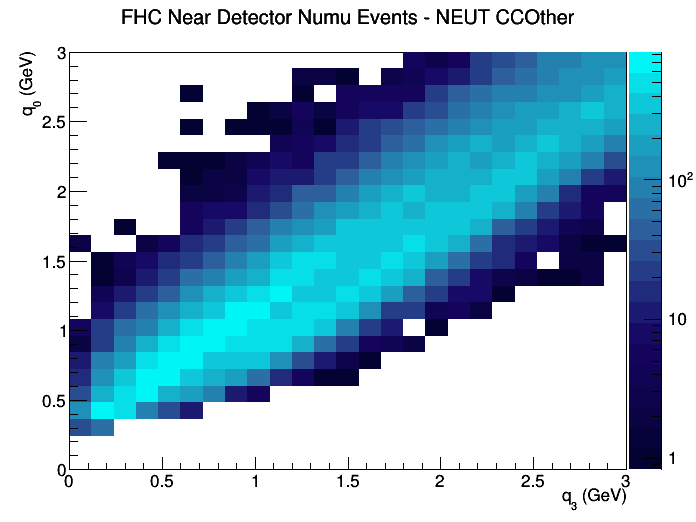
\includegraphics[width=\linewidth]{eff_q0_q3/FGT/CCOther_FHC_ND_numu_q3_q0_NEUT.png}
%\endminipage
%\minipage{.3\textwidth}
%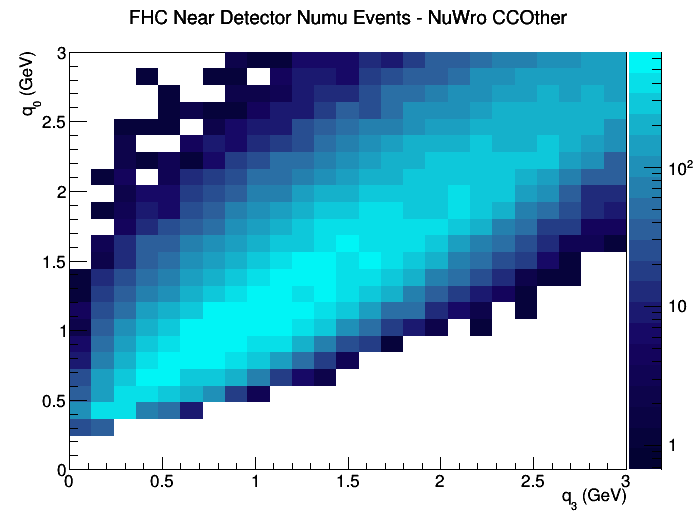
\includegraphics[width=\linewidth]{eff_q0_q3/FGT/CCOther_FHC_ND_numu_q3_q0_NuWro.png}
%\endminipage
%\caption{$q_0 \textrm{ - } q_3$ $\nu_{\mu}$ events using DUNE flux, Top Row: No Efficiencies applied, Bottom Row: FGT efficiencies applied to ND and LAr effiencies applied to FD. Right to Left: GENIE events distribution, NEUT events distribution, NuWro events distribution. The left $q_0 \textrm{ - } q_3$ region is being filled in after efficiencies are applied.}
%\label{fig:q0q3_numu_CCOther_events}
%\end{figure}
%\begin{figure}[h]
%\centering
%\minipage{.3\textwidth}
%\includegraphics[width=\linewidth]{Q2/nominal/CCOther_FHC_ND_numu_Q2_GENIE.png}
%\endminipage
%\minipage{.3\textwidth}
%\includegraphics[width=\linewidth]{Q2/nominal/CCOther_FHC_ND_numu_Q2_NEUT.png}
%\endminipage
%\minipage{.3\textwidth}
%\includegraphics[width=\linewidth]{Q2/nominal/CCOther_FHC_ND_numu_Q2_NuWro.png}
%\endminipage
%\newline
%\minipage{.3\textwidth}
%\includegraphics[width=\linewidth]{eff_Q2/FGT/CCOther_FHC_ND_numu_Q2_GENIE.png}
%\endminipage
%\minipage{.3\textwidth}
%\includegraphics[width=\linewidth]{eff_Q2/FGT/CCOther_FHC_ND_numu_Q2_NEUT.png}
%\endminipage
%\minipage{.3\textwidth}
%\includegraphics[width=\linewidth]{eff_Q2/FGT/CCOther_FHC_ND_numu_Q2_NuWro.png}
%\endminipage
%\caption{$Q^2$ events using DUNE flux, Top Row: No Efficiencies applied, Bottom Row: FGT efficiencies applied to ND and LAr effiencies applied to FD. Right to Left: GENIE events distribution, NEUT events distribution, NuWro events distribution. The low $Q^2$ region is being filled in after efficiencies are applied.}
%\label{fig:Q2_numu_CCOther_events}
%\end{figure}
%\FloatBarrier


\section{Reconstructed Energy}\label{sec:Reco}
%\subsection{Final State, Reconstructed Energy}

A framework for investigating variations in reconstructed energy calculations between different generators and ND configurations has been developed. %However, because it is calculated only by summing the final state energy (generator truth information), this is largely incomplete, and it serves only as a starting point for more robust studies. The full studies will include detector efficiencies and kinematic cuts to fully display the differences between models and configurations. 
Currently, the estimate for the incident neutrino energy is calculated by summing the total energy from final state leptons and pions (all charges) and the kinetic energy of final state protons after passing efficiencies through the data sets. All neutrons are assumed undetectable. 
This can be summed up in Equation~\ref{eq:ereco}:
%\begin{equation}
%E_{reco} = \Sigma {E_{lep}} + \Sigma E_{\pi} + \Sigma (E_{prot} - M_{prot})
%\label{eq:ereco}
%\end{equation}
where $E_{lep}$ is the energy of the outgoing lepton, $E_{\pi}$ is the energy of the pion, and $E_{prot}$ and $M_{prot}$ are the energy and mass of the proton.
%This is achieved by using the NUISANCE software package to reduce the output from various Monte Carlo neutrino event generators (including GENIE, NEUT, NUWRO, as well as the nuclear reaction and transport simulation software, GiBuu) into a common format that can easily be analyzed. 
%Work has begun to include tracking/PID efficiencies to accept or reject final state particles. So far, only the full information (barring $\pi^0$ efficiencies) for the FGT is available, but the inclusion of the LAr or GAr TPCs will be easily implemented. 

%\subsection{$E_\nu - E_{reco}$} 



\subsection{Neutron Multiplicities \& Energy}
\label{subsec:N_multiplicities_Energy}

Differences between models in the number of final state neutrons and the total energy into FS neutrons can largely affect reconstruction of neutrino energy. Large variations in reconstructed energy can arise due to missing energy caused by the inability to detect neutrons in the various models.  

\begin{table}
\centering
 \begin{tabular}{| l | c  c | c c |} 
 \hline
   Generator \& Interaction& $N_{neutron}>3 (\%)$ & $E_{neutron}>600 MeV/c (\%)$\\ 
    & \multicolumn{2}{|c|}{ND} & \multicolumn{2}{|c|}{FD} \\ \hline
   GENIE-CCQE & 13 & 2 & 13 & 2\\ 
   GENIE-2p2h & 28 & 1 & 29 & 2 \\ 
   GENIE-CC1$\pi$ & 17 & 21 & 18 & 25\\ 
   GENIE-CCOther & 24 & 17 & 24 & 19\\ \hline
   NEUT-CCQE & 1 & 0.8 & 1 & 0.7 \\ 
   NEUT-2p2h & 8 & 4 & 8 & 4\\ 
   NEUT-CC1$\pi$ & 9 & 21 & 9 & 23\\ 
   NEUT-CCOther & 9 & 18 & 11 & 21\\ \hline
   NuWro-CCQE & 4 & 2 & 3 & 2 \\ 
   NuWro-2p2h & 3 & 0.3 & 3 & 0.2\\ 
   NuWro-CC1$\pi$ & 30 & 22 & 34 & 27\\ 
   NuWro-CCOther & 33 & 20 & 38 & 26 \\ \hline
\end{tabular}
\caption{Percentage of events $N_{neutron}>3$ and $E_{neutron}>600 MeV/c$, broken down by generator and event type.  These cut offs where chosen to encompass most of the GENIE }
\label{tab:int_prob}
\end{table}


To investigate this, we have looked at GENIE, NEUT, and NUWRO to see if the different models showed a large difference in the neutron energy and multiplicity.  
This was done for CCQE-like, CC1$\pi$, 2p2h, and everything else (``Other'') interactions and neutrinos as well as anti-neutrinos.  
In all cases, the generators agreed rather well with each other even though there were some differences in the neutron multiplicity. 
These differences only account for a small fraction of the events, generally less than 10\%, as can be seen in Table~\ref{tab:int_prob}.
Figure~\ref{fig:Neutron_multi_2p2h_ND} shows an example of this for 2p2h neutrino events, while the other interaction modes can be found in Appendix~\ref{app:Neutron_Multiplicities}
  
\begin{figure}
\centering
\begin{subfigure}[b]{0.32\textwidth}
  \includegraphics[width=\textwidth]{nneutrons_v_total_ene/Nneutrons_Total_ENe_2p2h_GENIE_ND_numu.pdf}
\end{subfigure}
\begin{subfigure}[b]{0.32\textwidth}
  \includegraphics[width=\textwidth]{nneutrons_v_total_ene/Nneutrons_Total_ENe_2p2h_NEUT_ND_numu.pdf}
\end{subfigure}
\begin{subfigure}[b]{0.32\textwidth}
  \includegraphics[width=\textwidth]{nneutrons_v_total_ene/Nneutrons_Total_ENe_2p2h_NUWRO_ND_numu.pdf}
\end{subfigure}
\caption{The neutron multiplicity vs total neutron energy for 2p2h interactions for GENIE, NEUT, and NUWRO, respectively.  Even though they do show a different phase-space for the neutron multiplicity, they all agree where most of the energy lost to neutrons should be.  This is similar for other interaction types as well.}
\label{fig:Neutron_multi_2p2h_ND}
\end{figure}

Further more, the difference in the multiplicities between the generators becomes irrelevant after a ND to FD extraction, as can be seen in Figure~\ref{fig:Neutron_multi_2p2h_ND_FD}.
Here, the region where the most energy is lost agrees very well between the ND and FD for all generators and interaction types.
The areas with low statistics do show a disagreement, but very few events fall into this area.

\begin{figure}
\centering
\begin{subfigure}[b]{0.32\textwidth}
  \includegraphics[width=\textwidth]{nneutrons_v_total_ene/Nneutrons_Total_ENe_2p2h_GENIE_ND_FD_numu_norm.pdf}
\end{subfigure}
\begin{subfigure}[b]{0.32\textwidth}
  \includegraphics[width=\textwidth]{nneutrons_v_total_ene/Nneutrons_Total_ENe_2p2h_NEUT_ND_FD_numu_norm.pdf}
\end{subfigure}
\begin{subfigure}[b]{0.32\textwidth}
  \includegraphics[width=\textwidth]{nneutrons_v_total_ene/Nneutrons_Total_ENe_2p2h_NUWRO_ND_FD_numu_norm.pdf}
\end{subfigure}
\caption{The ratio of the ND to the FD for neutron multiplicity vs total neutron energy for 2p2h interactions for GENIE, NEUT, and NUWRO, respectively.  In the area where the largest amount of energy is lost to neutrons, low multiplicity and low energy, the agreement between the ND and FD is almost perfect.} 
\label{fig:Neutron_multi_2p2h_ND_FD}
\end{figure}

Care should still be taken when calculating the neutrino energy of the event if only a calorimetric approach is used, as is the case in this document.
This is because as much as 50\% of the energy can be taken away by the neutron in CCQE-like events.
Even for 2p2h events, as shown in Figure~\ref{fig:Neutron_multi_ene_enu_2p2h_ND}, it can be as high as 30\%.
The other interaction modes and anti-neutrino events can also be found in Appendix~\ref{app:Neutron_Multiplicities} and have a smaller fraction.

\begin{figure}
\centering
\begin{subfigure}[b]{0.32\textwidth}
  \includegraphics[width=\textwidth]{nneutrons_ene_enu/Nneutrons_Enu_true_2p2h_GENIE_ND_numu_norm.pdf}
\end{subfigure}
\begin{subfigure}[b]{0.32\textwidth}
  \includegraphics[width=\textwidth]{nneutrons_ene_enu/Nneutrons_Enu_true_2p2h_NEUT_ND_numu_norm.pdf}
\end{subfigure}
\begin{subfigure}[b]{0.32\textwidth}
  \includegraphics[width=\textwidth]{nneutrons_ene_enu/Nneutrons_Enu_true_2p2h_NUWRO_ND_numu_norm.pdf}
\end{subfigure}
\caption{Neutron multiplicity vs total neutron energy divide by the neutrino energy for 2p2h interactions from GENIE, NEUT, and NUWRO, respectively.  For low multiplicity, the neutron carries away a significant fraction of the neutrino energy.} 
\label{fig:Neutron_multi_ene_enu_2p2h_ND}
\end{figure}
\FloatBarrier

Missing neutrons can effect the neutrino energy reconstruction, which is especially important for neutrino oscillation studies which require an exact energy.
However, much of the effect of these missing neutrons can be taken into account with the Near to Far extrapolation.
At the moment the difference between the models seem to be OK for these analyses given a Near to Far ratio.
Future investigations will include the ability for errors in GENIE to cover the differences between the models. 
 

\subsection{Proton/Pion Multiplicity and Momentum}
\label{subsec:Particle_multiplicities_momentum}

Similar to the neutron multiplicity and energy studies, proton and pion multiplicities offer insight into the coupling of the detector configurations with variations in FSI models as well as the energy reconstruction capabilities of the different detector configurations. 
The total momentum of the particles gives us a proxy for the energy into the FS protons or pions as well as a direct link to detector efficiency effects.  
For these studies, the 3-momentum of the final state protons are summed. 
The magnitude is then plotted against the multiplicity for the specific particle type. 
This was done for the final state particles in true-CCQE, true-2p2h, CC0$\pi$, CC1$\pi$, and CCOther. It was first done without efficiencies applied so we can look at the effects of the FSI models. It was also done with all 3 ND configuration efficiencies and the LAr FD efficiencies so we can investigate the effects of the different ND configurations and how the couple to the FD.
As the efficiencies for pions are currently unknown for the LAr and GAr, we will only consider the protons in the current iteration of this note. 

To show the difference in the FSI models, Figure~\ref{fig:proton_multiplicity_2p2h} shows the proton multiplicity vs total proton momentum for 2p2h interactions. 
2p2h models where chosen as they have the smallest phase space in this projection and therefore show the differences the best, but all interaction types have been investigated and can be found in Appendix~\ref{app:proton_meultiplicty}.
From this, one can see that there is a difference between the FSI models.  
Particularly, GENIE prefers to have more proton multiplicity compared to NEUT and NuWro.
It also has lower total momentum for these protons when compared to the other two.
 
\begin{figure}[h]
\centering
\begin{subfigure}[b]{0.32\textwidth}
\includegraphics[width=\linewidth]{N_P/nominal/protons/2p2h_FHC_ND_numu_N_P_GENIE.png}
\end{subfigure}
\begin{subfigure}[b]{0.32\textwidth}
\includegraphics[width=\linewidth]{N_P/nominal/protons/2p2h_FHC_ND_numu_N_P_NEUT.png}
\end{subfigure}
\begin{subfigure}[b]{0.32\textwidth}
\includegraphics[width=\linewidth]{N_P/nominal/protons/2p2h_FHC_ND_numu_N_P_NuWro.png}
\end{subfigure}
\caption{The proton multiplicity as a function of total proton momentum for 2p2h interaction in GENIE, NEUT, and NuWro, respectively. There is a clear difference in phase space with GENIE having both higher proton multiplicity and lower total momentum.}
\label{fig:proton_multiplicity_2p2h}
\end{figure}

Unlike with the neutron multiplicity, the differences between the models is important as the a Near to Far extrapolation does not hold.  
Figure~\ref{proton_multiplicity_2p2h_NF} shows this with variations of 20-30\% in the regions where the most events are.  
The exact reason for this discrepancy is unclear.
It could be attributed to the plot only includes the total momentum of all protons, with it being possible that one or two protons take away the most energy and the highest momentum protons would agree between the two detectors.
This is something that needs to be investigated further in future works.  

\begin{figure}[h]
\centering
\begin{subfigure}[b]{0.32\textwidth}
\includegraphics[width=\linewidth]{N_P/nominal/protons/ratios/2p2h_GENIE_numu_NF_N_P.png}
\end{subfigure}
\begin{subfigure}[b]{0.32\textwidth}
\includegraphics[width=\linewidth]{N_P/nominal/protons/ratios/2p2h_NEUT_numu_NF_N_P.png}
\end{subfigure}
\begin{subfigure}[b]{0.32\textwidth}
\includegraphics[width=\linewidth]{N_P/nominal/protons/ratios/2p2h_NuWro_numu_NF_N_P.png}
\end{subfigure}
\caption{The ND/FD of proton multiplicity as a function of total proton momentum for 2p2h interaction in GENIE, NEUT, and NuWro, respectively. In the region with the most events, there are variations of up to 20\%}
\label{fig:proton_multiplicity_2p2h_NF}
\end{figure}

Once detector efficiencies are added in, there is even a greater difference in the Near to Far ratio.  
Figure~\ref{fig:proton_multiplicity_2p2h_NF_eff} shows these striking differences.  
The top row shows the Near to Far ratio for the FGT to a LAr far detector.  
In the region of interest the differences are 100\% and greater.
The middle row shows the high pressure GAr TPC, with differences again ranging from 20-100\%.
The last row shows the LAr TPC, and unsurprisingly, gives the best agreement. 
Event then though, differences of up to 20\% exist, arising most likely due to the different flux at each detector. 

These plots show the importance of not just the FSI model in use but also the detector's threshold to measure protons. 
The FGT, which has the most realistic thresholds and therefore the ones most unlike the LAr far detector, shows just how important this can be.
It is expected pions will have an even larger impact than the protons due to there re-interactions with the nucleus.  
This needs to be confirmed and will be shown in updates to this document. 

\begin{figure}[h]
\centering
\begin{subfigure}[b]{0.32\textwidth}
\includegraphics[width=\linewidth]{eff_N_P/FGT/protons/ratios/2p2h_GENIE_numu_NF_N_P.png}
\end{subfigure}
\begin{subfigure}[b]{0.32\textwidth}
\includegraphics[width=\linewidth]{eff_N_P/FGT/protons/ratios/2p2h_NEUT_numu_NF_N_P.png}
\end{subfigure}
\begin{subfigure}[b]{0.32\textwidth}
\includegraphics[width=\linewidth]{eff_N_P/FGT/protons/ratios/2p2h_NuWro_numu_NF_N_P.png}
\end{subfigure}

\begin{subfigure}[b]{0.32\textwidth}
\includegraphics[width=\linewidth]{eff_N_P/GAr/protons/ratios/2p2h_GENIE_numu_NF_N_P.png}
\end{subfigure}
\begin{subfigure}[b]{0.32\textwidth}
\includegraphics[width=\linewidth]{eff_N_P/GAr/protons/ratios/2p2h_NEUT_numu_NF_N_P.png}
\end{subfigure}
\begin{subfigure}[b]{0.32\textwidth}
\includegraphics[width=\linewidth]{eff_N_P/GAr/protons/ratios/2p2h_NuWro_numu_NF_N_P.png}
\end{subfigure}

\begin{subfigure}[b]{0.32\textwidth}
\includegraphics[width=\linewidth]{eff_N_P/LAr/protons/ratios/2p2h_GENIE_numu_NF_N_P.png}
\end{subfigure}
\begin{subfigure}[b]{0.32\textwidth}
\includegraphics[width=\linewidth]{eff_N_P/LAr/protons/ratios/2p2h_NEUT_numu_NF_N_P.png}
\end{subfigure}
\begin{subfigure}[b]{0.32\textwidth}
\includegraphics[width=\linewidth]{eff_N_P/LAr/protons/ratios/2p2h_NuWro_numu_NF_N_P.png}
\end{subfigure}
\caption{The ND/FD of proton multiplicity as a function of total proton momentum for 2p2h interactions. The left hand columns show GENIE, and middle column shows NEUT, and the right hand column shows NuWro. The top row has the FGT efficiencies applied for the ND, the middle row has the high pressure GAr TPC efficiencies, while the last row has the LAr TPC efficiencies for the ND.  All of these use LAr efficiencies for the FD.}
\label{fig:proton_multiplicity_2p2h_NF_eff}
\end{figure}
%\FloatBarrier


\subsection{Difference from True Neutrino Energy}
\label{subsec:EDiff}
The studies in Sections~\ref{subsec:N_multiplicities_Energy} and ~\ref{subsec:Particle_multiplicities_momentum} highlight the differences in the generators' FSI behavior as well as the different abilities of the various detector configurations to reconstruct final state energy. This section studies the overall change we see to $E_{reco}$ - defined in Equation~\ref{eq:ereco} - as we apply detector efficiencies. To do this, the difference between true and reconstructed neutrino energy from each generator is plotted. This is first done for a 'perfect' near detector - one in which we assume all particles except neutrons are accepted. Next, it is done for each ND configuration - FGT, simple LAr, and simple GAr. % - and the simpe LAr FD. 
Each distribution is normalized to 1 so the y-axis serves as the relative event rate. 
%True-CCQE and true-2p2h are both defined as MC-level CCQE/2p2h interaction - with 1 reconstructed lepton if efficiencies are applied. CC0$\pi$ is defined as 0 $\pi^{\pm}$, 1 lepton, and any number of protons and $\pi^0$ after reconstruction. CC1$\pi$ is defined as 1 $\pi^{\pm}$, 1 lepton, and any number of protons and $\pi^0$ after reconstruction. Finally, CCOther is defined as any final state with 1 lepton and any number of hadrons reconstructed.

%The 'perfect' ND plots give insight into the FSI behavior of the different generators. Differences between true and reconstructed energy arise from 2 effects. The first is the FSI behavior, in which some of the neutrino energy is imparted to protons and pions that are reabsorbed in the nucleus in the generator MC. This results in some of the reconstructed energy being lost, as we only sum up what is in the final state and is visible, and is the focus of Section~\ref{subsec:Particle_multiplicities_momentum}. Further discrepancy arises from neutrons which are either reabsorbed in the nucleus or are present in the final state, but are invisible to the detector. This being the focus of Section~\ref{subsec:N_multiplicities_Energy}. 

For $\nu_\mu$, all 3 generators behave similarly in the perfect ND for CCQE, 2p2h, CC0$\pi$, and CC1$\pi$. This is shown for CCQE in the left plot of Figure~\ref{fig:numu_Etrue_ereco_perfect}. Meanwhile, NuWro CCOther is slightly different to NEUT and GENIE, as seen in the right plot of the same figure. The other reactions can be found in Appendix~\ref{app:Ereco_app}. 

However, for $\overline{\nu}_\mu$ in the perfect ND, NuWro now differs significantly from NEUT and GENIE for CCQE, 2p2h, and CC0$\pi$, while all 3 generators behave similarly for CC1$\pi$ and CCOther. This is shown for 2p2h and CCOther in Figure~\ref{fig:numubar_Etrue_ereco_perfect}.

Future work will be conducted to determine if GENIE FSI errors are able to cover the variations between these generators within the perfect ND.
%In $\nu_\mu$ mode: for all reaction types except CCOther, all three generators seem to have similar differences in all detector configurations. This is evident in Figure~\ref{fig:numu_Etrue_ereco_FGT_CCQE_and_CCOther} - which includes CCQE and CCOther interactions in the ND with FGT efficiencies - and the figures in Appendix~\ref{app:Ereco_app}. For CCOther, all three generators appear to have a long tail extending to high discrepancy regions - well past that of CCQE for example - though NuWro has a higher amount of events in the $\Delta E$ = 0.5 GeV to 2 GeV region. 
\begin{figure}[h]
\centering
\minipage{.5\textwidth}
\includegraphics[width=\linewidth]{Ereco_Etrue/numu_perfect_ND_CCQE.png}
\endminipage
\minipage{.5\textwidth}
\includegraphics[width=\linewidth]{Ereco_Etrue/numu_perfect_ND_CCOther.png}
\endminipage
\caption{Difference between true and reconstructed neutrino energy in the 'perfect' ND. Left: $nu_\mu$ CCQE, Right: CCOther. All 3 generators behave similarly for CCQE. For CCOther, NEUT and GENIE have similar behavior, while NuWro slightly differs.}
\label{fig:numu_Etrue_ereco_perfect}
\end{figure}
\begin{figure}[h]
\centering
\minipage{.5\textwidth}
\includegraphics[width=\linewidth]{Ereco_Etrue/numubar_perfect_ND_2p2h.png}
\endminipage
\minipage{.5\textwidth}
\includegraphics[width=\linewidth]{Ereco_Etrue/numubar_perfect_ND_CCOther.png}
\endminipage
\caption{Difference between true and reconstructed neutrino energy in the 'perfect' ND. Left: 2p2h $\overline{\nu}_\mu$, Right: CCOther. NuWro differs from NEUT and GENIE in 2p2h, while all generators are similar for CCOther.}
\label{fig:numubar_Etrue_ereco_perfect}
\end{figure}
\FloatBarrier

After applying detector efficiencies, the discrepancy between true and reconstructed neutrino energy changes only slightly as seen in Figure~\ref{fig:numu_2p2h_Etrue_ereco_allND}. Here, we show the $\nu_\mu$ 2p2h distributions with the perfect, simple LAr, simple GAr, and FGT ND. The other reaction modes can be found in Appendix~\ref{app:Ereco_app}. Keeping in mind that the simple GAr and LAr only include thresholds (100 and 200 MeV respectively) for protons, comparing these configurations to the perfect ND shows that a simple proton threshold has little effect on the ability to reconstruct the true neutrino energy. This is in contrast to the conclusion of Section~\ref{subsec:Particle_multiplicities_momentum}. Though applying proton thresholds appears to have a drastic effect when looking at the multiplicity and momentum distributions, it is shown here that this has only a small effect on the reconstructed neutrino energy. Future work will include a more reasonable description of the proton efficiencies, as well as efficiency descriptions for the other final state particles, within these two detectors to see if any larger effect arises.

Applying the FGT efficiencies has a slightly more noticeable effect, as can be seen in the bottom right plot of Figure~\ref{fig:numu_2p2h_Etrue_ereco_allND}. This motivates further investigation into both the relative effect of applying a more complete description of proton efficiencies and including efficiencies for other final state particles. Additional studies include applying the FGT efficiencies for each particle individually in order to see each effect independently. 
\begin{figure}[h]
\centering
\minipage{.5\textwidth}
\includegraphics[width=\linewidth]{Ereco_Etrue/numu_perfect_ND_2p2h.png}
\endminipage
\minipage{.5\textwidth}
\includegraphics[width=\linewidth]{Ereco_Etrue/numu_LAr_2p2h.png}
\endminipage
\newline
\minipage{.5\textwidth}
\includegraphics[width=\linewidth]{Ereco_Etrue/numu_GAr_2p2h.png}
\endminipage
\minipage{.5\textwidth}
\includegraphics[width=\linewidth]{Ereco_Etrue/numu_FGT_2p2h.png}
\endminipage
\caption{Difference between true and reconstructed neutrino energy for $\nu_\mu$ 2p2h. Top Left: Perfect ND, Top Right: Simple LAr ND. Bottom Left: Simple GAr ND, Bottom Right: FGT ND. There exists only small differences when applying simple LAr and GAr proton thresholds. There is a slightly more noticeable effect when applying a more complete FGT description.}
\label{fig:numu_2p2h_Etrue_ereco_allND}
\end{figure}
\FloatBarrier
% \subsection{Nucleon multiplicity vs. W}
% \label{sec:Nucleon_multi_w}
% Differences in mapping from $E_{reco}$ to true variables can arise from shape differences in nucleon multiplicities vs. W distributions. 
% These distributions can also show where in the phase space most of the events shown in Section~\ref{sec:N_multiplicities_Energy} and Section~\ref{sec:Particle_multiplicities_Energy} exist.  A first look of this is shown in this section.

% \subsubsection{Neutrons vs W}

% Apart from the difference in neutron multiplicity discussed in Section~\ref{sec:N_multiplicities_Energy}, the exact phase space of these event in the neutron/W plane is slightly different.  
% This is most pronounced for 2p2h events, as can be seen in Figure~\ref{Neutron_w_2p2h_ND}. 
% The width of NEUT's peak is broader then GENIE's or NUWRO's while NUWRO allows for much higher W's.

% \begin{figure}
% \centering
% \begin{subfigure}[b]{0.32\textwidth}
%   \includegraphics[width=\textwidth]{nneutrons_w/Nneutrons_W_nuc_rest_2p2h_GENIE_ND_numu.pdf}
% \end{subfigure}
% \begin{subfigure}[b]{0.32\textwidth}
%   \includegraphics[width=\textwidth]{nneutrons_w/Nneutrons_W_nuc_rest_2p2h_NEUT_ND_numu.pdf}
% \end{subfigure}
% \begin{subfigure}[b]{0.32\textwidth}
%   \includegraphics[width=\textwidth]{nneutrons_w/Nneutrons_W_nuc_rest_2p2h_NUWRO_ND_numu.pdf}
% \end{subfigure}
% \caption{The neutron multiplicity vs W for 2p2h interactions from GENIE, NEUT, and NUWRO, respectively.  It can be seen that all three event generators have the peak of the distribution at the same place, but NEUT's peak is much broader while NUWRO allows for much higher W's.}
% \label{fig:Neutron_w_2p2h_ND}
% \end{figure}

% However, Figure~\ref{fig:Neutron_w_2p2h_ND_FD} shows that the differences are not so important if a Near to Far extrapolation is used, as both the ND and FD have simular responses.
% To see if the different models could have a larger affect on the physics results, we have taken a double ratio of the ND/FD and the different generators to GENIE.  
% Interestingly, Figure~\ref{fig:Neutron_w_2p2h_ND_FD_GENIE} indicates that there would not be large affect if a few perecent difference between the models is acceptable.

% \begin{figure}
% \centering
% \begin{subfigure}[b]{0.32\textwidth}
%   \includegraphics[width=\textwidth]{nneutrons_w/Nneutrons_W_nuc_rest_2p2h_GENIE_ND_FD_numu_norm.pdf}
% \end{subfigure}
% \begin{subfigure}[b]{0.32\textwidth}
%   \includegraphics[width=\textwidth]{nneutrons_w/Nneutrons_W_nuc_rest_2p2h_NEUT_ND_FD_numu_norm.pdf}
% \end{subfigure}
% \begin{subfigure}[b]{0.32\textwidth}
%   \includegraphics[width=\textwidth]{nneutrons_w/Nneutrons_W_nuc_rest_2p2h_NUWRO_ND_FD_numu_norm.pdf}
% \end{subfigure}
% \caption{The ND/FD ratio of neutron multiplicity vs W for 2p2h interactions from GENIE, NEUT, and NUWRO, respectively.  The effects of the different phase space seen in Figure~\ref{fig:Neutron_w_2p2h_ND} is not great if a ND ro FD extropolation is used.  This can be seen by the ratio being very close to one at the peak of Figure~\ref{fig:Neutron_w_2p2h_ND} distribution.}
% \label{fig:Neutron_w_2p2h_ND_FD}
% \end{figure}

% These results are also true for protons and pions, though pions have a much lower multiplicity.  
% Those results, along with other interactions can be found in Appendix~\ref{app:Nucleon_W}.

% \begin{figure}
% \centering
% \begin{subfigure}[b]{0.32\textwidth}
%   \includegraphics[width=\textwidth]{nneutrons_w/Nneutrons_W_nuc_rest_2p2h_GENIE_NEUT_ND_FD_numu_norm.pdf}
% \end{subfigure}
% \begin{subfigure}[b]{0.32\textwidth}
%   \includegraphics[width=\textwidth]{nneutrons_w/Nneutrons_W_nuc_rest_2p2h_GENIE_NUWRO_ND_FD_numu_norm.pdf}
% \end{subfigure}
% \caption{The double ratio of ND/FD and the event generators to GENIE of the neutron multiplicity vs W for 2p2h interactions.  Despite the differences seen in the W distributions, the double ratio shows suprisingly good agreement between the generators, indicating that the different models should not have a large impact on the final results.}
% \label{fig:Neutron_w_2p2h_ND_FD_GENIE}
% \end{figure}

% \subsubsection{Protons vs W}

% In the last section we saw a differnce in the phase space between the different generators.  
% Now we will show an instance where the phase space is almost the same but there is a large difference between the ND and FD.  
% Though here we are only showing the results for CC1$\pi$ via protons, the results are the same for CC-Other (anything not CCQE, CC1$\pi$, or 2p2h), and neutrons along with pions.
% Figure~\ref{fig:Proton_w_res_ND} shows that GENIE, NEUT, and NUWRO have very similar distributions.

% \begin{figure}
% \centering
% \begin{subfigure}[b]{0.32\textwidth}
%   \includegraphics[width=\textwidth]{nprotons_w/Nprotons_W_nuc_rest_res_GENIE_ND_numu.pdf}
% \end{subfigure}
% \begin{subfigure}[b]{0.32\textwidth}
%   \includegraphics[width=\textwidth]{nprotons_w/Nprotons_W_nuc_rest_res_NEUT_ND_numu.pdf}
% \end{subfigure}
% \begin{subfigure}[b]{0.32\textwidth}
%   \includegraphics[width=\textwidth]{nprotons_w/Nprotons_W_nuc_rest_res_NUWRO_ND_numu.pdf}
% \end{subfigure}
% \caption{The proton multiplicity vs W for CC1$\pi$ interactions from GENIE, NEUT, and NUWRO, respectively.  It can be seen that all three event generators have the peak of their distribution at the same place and are almost identical}
% \label{fig:Proton_w_res_ND}
% \end{figure}

% If a Near to Far detector extrapolation is used, however, there are much larger differences in region of most interest. 
% Figure~\ref{fig:Proton_w_res_ND_FD} shows that there is a difference between the two detectors between 20\% and 40\% at the peak of the distribution.  
% There is also a clear difference in lower W values compared to higher W values. 


% \begin{figure}
% \centering
% \begin{subfigure}[b]{0.32\textwidth}
%   \includegraphics[width=\textwidth]{nprotons_w/Nprotons_W_nuc_rest_res_GENIE_ND_FD_numu_norm.pdf}
% \end{subfigure}
% \begin{subfigure}[b]{0.32\textwidth}
%   \includegraphics[width=\textwidth]{nprotons_w/Nprotons_W_nuc_rest_res_NEUT_ND_FD_numu_norm.pdf}
% \end{subfigure}
% \begin{subfigure}[b]{0.32\textwidth}
%   \includegraphics[width=\textwidth]{nprotons_w/Nprotons_W_nuc_rest_res_NUWRO_ND_FD_numu_norm.pdf}
% \end{subfigure}
% \caption{The ND/FD ratio of the proton multiplicity vs W for CC1$\pi$ interactions from GENIE, NEUT, and NUWRO, respectively.  Unlike with 2p2h events shown for neutrons, there are clear differences between the ND and FD.  At the peak of the distribution this is between 20\% and 40\%.  Furthermore, there is a clear difference between W values below 2000 and ones above it.}
% \label{fig:Proton_w_res_ND_FD}
% \end{figure}

% We can again see if the different models could have a larger affect on the physics results, by taking the double ratio as we did before.
% Simular to before, Figure~\ref{fig:Proton_w_res_ND_FD_GENIE} indicates that there would not be large affect if a few perecent difference between the models is acceptable.
% In the region of interest, the difference between GENIE and NEUT is negligable while it is small compared to NUWRO.


% \begin{figure}
% \centering
% \begin{subfigure}[b]{0.32\textwidth}
%   \includegraphics[width=\textwidth]{nprotons_w/Nprotons_W_nuc_rest_res_GENIE_NEUT_ND_FD_numu_norm.pdf}
% \end{subfigure}
% \begin{subfigure}[b]{0.32\textwidth}
%   \includegraphics[width=\textwidth]{nprotons_w/Nprotons_W_nuc_rest_res_GENIE_NUWRO_ND_FD_numu_norm.pdf}
% \end{subfigure}
% \caption{The double ratio of ND/FD and the event generators to GENIE of the proton multiplicity vs W for CC1$\pi$ interactions.  Despite the differences seen in the single ratio, the double ratio shows suprisingly good agreement between the generators}
% \label{fig:Proton_w_res_ND_FD_GENIE}
% \end{figure}



\section{Future Work}\label{sec:Future}

The above studies need to be furthered and expanded upon to successfully arrive at useful conclusions on ND configuration choice. 

\begin{itemize}

\item Improved statistics.
	\begin{itemize}
		\item This can be easily and quickly achieved.
	\end{itemize}
\item Investigate origins of high-$Q^2$ variations
	\begin{itemize}
		\item Is this FSI or detector effects?
	\end{itemize}
\item Extend studies to include LAr and GAr efficiency and acceptance information when available.
\item Extend final state studies into proton multiplicity vs. energy, and include pions when efficiencies are available.
\item Study the ability for GENIE FSI errors to cover differences between generators and final state energy.
\item Study the effect on the reconstructed neutrino energy of applying efficiencies to each final state particle independently.
%\item Current uncertainties are invariant of target choice. Need to extend studies to include Calcium-40 target for FGT studies
%\item Include a mapping of $E_{true}$ to $E_{reco}$ along with $y_{true}$ to $y_{reco}$ and investigate differences between configurations.

\end{itemize}


%\subsection{Ereco, yreco}
%An additional study to be commenced is the mapping from Ereco \& yreco into other kinematic variables (i.e. $Q^2$, $q_0$ vs. $q_3$), and the ability to similarly map model variations.
\appendix

%\subfile{Appendix_Neutron_Multi.tex}
%
%\subfile{Appendix_Nucleon_Multi.tex}
%
%\subfile{DUNE_appendix_Ereco_plots.tex}
%\subfile{DUNE_appendix_Q2_plots.tex}
%\subfile{DUNE_appendix_q0_q3_plots.tex}
%\subfile{DUNE_appendix_N_P_plots_protons.tex}

%\subfile{DUNE_appendix_eff_plots.tex}

\begin{thebibliography}{7}

\bibitem{DUNE_CDR1}
The DUNE Collaboration
\textit{Long-Baseline Neutrino Facility (LBNF) and Deep Underground Neutrino Experiment (DUNE) Conceptual Design Report Volume 1: The LBNF and DUNE Projects}
arXiv:1601.05471v1

\bibitem{DUNE_review}
Maury Goodman
\textit{The Deep Underground Neutrino Experiment}
Advances in High Energy Physics, vol. 2015, Article ID 256351, 9 pages, 2015. doi:10.1155/2015/256351

\bibitem{GENIE}
Andreopoulos, C. \textit{et al}.
\textit{The GENIE Neutrino Monte Carlo Generator}.
Nucl.Instrum.Meth. A614 (2010) 87-104 arXiv:0905.2517 [hep-ph] FERMILAB-PUB-09-418-CD

\bibitem{NEUT}
Hayato, Yoshinari 
\textit{A neutrino interaction simulation program library NEUT}.
Acta Phys.Polon. B40 (2009) 2477-2489

\bibitem{NUWRO}
T. Golan, J.T. Sobczyk, J. Zmuda
\textit{NuWro: the Wrocław Monte Carlo Generator of Neutrino Interactions}.
Nuclear Physics B - Proceedings Supplements 229 (2012) 499

\bibitem{NUISANCE}
P. Stowell, C. Wret, C. Wilkinson, L. Pickering, S. Cartwright, Y. Hayato, K. Mahn, K.S. McFarland, J. Sobczyk, R. Terri, L. Thompson, M.O. Wascko, Y. Uchida
\textit{NUISANCE: a neutrino cross-section generator tuning and comparison framework}
arXiv:1612:07393v2

\bibitem{DUNE_osc}
T. Alion, \textit{et al.}
\textit{Experiment Simulation Configurations Used in DUNE CDR}
arXiv:1606.09550

\bibitem{VALOR}
Andreopoulos, \textit{et al.}
\textit{VALOR DUNE Joint Oscillation and Systematics Constraint Fit}


\end{thebibliography}

\end{document}




